% -*- mode: latex; coding: utf-8 -*-
\newcommand{\drawblock}[5]{% PARAMETERS: COLOR, CORNERCOORDS, SIZE
% TOP SIDE
\color{#1!55}
\pgfmoveto{\pgfrelative{\pgfxyz(#2,#3,#4)}{\pgfxyz(0,#5,0)}}
\pgflineto{\pgfrelative{\pgfxyz(#2,#3,#4)}{\pgfxyz(#5,#5,0)}}
\pgflineto{\pgfrelative{\pgfxyz(#2,#3,#4)}{\pgfxyz(#5,#5,#5)}}
\pgflineto{\pgfrelative{\pgfxyz(#2,#3,#4)}{\pgfxyz(0,#5,#5)}}
\pgflineto{\pgfrelative{\pgfxyz(#2,#3,#4)}{\pgfxyz(0,#5,0)}}
\pgffill
\color{black}
\pgfmoveto{\pgfrelative{\pgfxyz(#2,#3,#4)}{\pgfxyz(0,#5,0)}}
\pgflineto{\pgfrelative{\pgfxyz(#2,#3,#4)}{\pgfxyz(#5,#5,0)}}
\pgflineto{\pgfrelative{\pgfxyz(#2,#3,#4)}{\pgfxyz(#5,#5,#5)}}
\pgflineto{\pgfrelative{\pgfxyz(#2,#3,#4)}{\pgfxyz(0,#5,#5)}}
\pgflineto{\pgfrelative{\pgfxyz(#2,#3,#4)}{\pgfxyz(0,#5,0)}}
\pgfstroke
% RIGHT SIDE
\color{#1!65}
\pgfmoveto{\pgfrelative{\pgfxyz(#2,#3,#4)}{\pgfxyz(#5,0,0)}}
\pgflineto{\pgfrelative{\pgfxyz(#2,#3,#4)}{\pgfxyz(#5,#5,0)}}
\pgflineto{\pgfrelative{\pgfxyz(#2,#3,#4)}{\pgfxyz(#5,#5,#5)}}
\pgflineto{\pgfrelative{\pgfxyz(#2,#3,#4)}{\pgfxyz(#5,0,#5)}}
\pgflineto{\pgfrelative{\pgfxyz(#2,#3,#4)}{\pgfxyz(#5,0,0)}}
\pgffill
\color{black}
\pgfmoveto{\pgfrelative{\pgfxyz(#2,#3,#4)}{\pgfxyz(#5,0,0)}}
\pgflineto{\pgfrelative{\pgfxyz(#2,#3,#4)}{\pgfxyz(#5,#5,0)}}
\pgflineto{\pgfrelative{\pgfxyz(#2,#3,#4)}{\pgfxyz(#5,#5,#5)}}
\pgflineto{\pgfrelative{\pgfxyz(#2,#3,#4)}{\pgfxyz(#5,0,#5)}}
\pgflineto{\pgfrelative{\pgfxyz(#2,#3,#4)}{\pgfxyz(#5,0,0)}}
\pgfstroke
%FRONT
\color{#1!99}
\pgfmoveto{\pgfxyz(#2,#3,#4)}
\pgflineto{\pgfrelative{\pgfxyz(#2,#3,#4)}{\pgfxyz(#5,0,0)}}
\pgflineto{\pgfrelative{\pgfxyz(#2,#3,#4)}{\pgfxyz(#5,#5,0)}}
\pgflineto{\pgfrelative{\pgfxyz(#2,#3,#4)}{\pgfxyz(0,#5,0)}}
\pgflineto{\pgfxyz(#2,#3,#4)}
\pgffill
\color{black}
\pgfmoveto{\pgfxyz(#2,#3,#4)}
\pgflineto{\pgfrelative{\pgfxyz(#2,#3,#4)}{\pgfxyz(#5,0,0)}}
\pgflineto{\pgfrelative{\pgfxyz(#2,#3,#4)}{\pgfxyz(#5,#5,0)}}
\pgflineto{\pgfrelative{\pgfxyz(#2,#3,#4)}{\pgfxyz(0,#5,0)}}
\pgflineto{\pgfxyz(#2,#3,#4)}
\pgfstroke
}

\newcommand{\RsGsB}{\begin{pgfpicture}{0.5mm}{0.5mm}{9mm}{3.75mm}
\pgfsetxvec{\pgfpoint{0.4cm}{0cm}}
\pgfsetyvec{\pgfpoint{0cm}{0.4cm}}
\pgfsetzvec{\pgfpoint{0.15cm}{0.15cm}}
\drawblock{red}{0}{0}{0}{0.75}
\drawblock{green}{0.75}{0}{0}{0.75}
\drawblock{blue}{1.5}{0}{0}{0.75}
\end{pgfpicture}
}

\newcommand{\twostacksA}[3]{\begin{pgfpicture}{0.5mm}{0.5mm}{0.6cm}{0.675cm}
\pgfsetxvec{\pgfpoint{0.4cm}{0cm}}
\pgfsetyvec{\pgfpoint{0cm}{0.4cm}}
\pgfsetzvec{\pgfpoint{0.15cm}{0.15cm}}
\drawblock{#2}{0}{0}{0}{0.75}
\drawblock{#1}{0}{0.75}{0}{0.75}
\drawblock{#3}{0.75}{0}{0}{0.75}
\end{pgfpicture}
}

\newcommand{\twostacksB}[3]{\begin{pgfpicture}{0.5mm}{0.5mm}{0.6cm}{0.675cm}
\pgfsetxvec{\pgfpoint{0.4cm}{0cm}}
\pgfsetyvec{\pgfpoint{0cm}{0.4cm}}
\pgfsetzvec{\pgfpoint{0.15cm}{0.15cm}}
\drawblock{#1}{0}{0}{0}{0.75}
\drawblock{#3}{0.75}{0}{0}{0.75}
\drawblock{#2}{0.75}{0.75}{0}{0.75}
\end{pgfpicture}
}

\newcommand{\onestack}[3]{\begin{pgfpicture}{0.5mm}{0.5mm}{3mm}{9.75mm}
\pgfsetxvec{\pgfpoint{0.4cm}{0cm}}
\pgfsetyvec{\pgfpoint{0cm}{0.4cm}}
\pgfsetzvec{\pgfpoint{0.15cm}{0.15cm}}
\drawblock{#3}{0}{0}{0}{0.75}
\drawblock{#2}{0}{0.75}{0}{0.75}
\drawblock{#1}{0}{1.5}{0}{0.75}
\end{pgfpicture}
}

\newcommand{\RGsB}{\twostacksA{red}{green}{blue}}

\newcommand{\RBsG}{\twostacksB{green}{red}{blue}}
\newcommand{\RBsGr}{\twostacksA{red}{blue}{green}}

\newcommand{\BRsG}{\twostacksA{blue}{red}{green}}
\newcommand{\BRsGr}{\twostacksB{green}{blue}{red}}

\newcommand{\RsBG}{\twostacksB{red}{blue}{green}}

\newcommand{\GRsB}{\twostacksA{green}{red}{blue}}
\newcommand{\RsGB}{\twostacksB{red}{green}{blue}}

\newcommand{\RGB}{\onestack{red}{green}{blue}}
\newcommand{\RBG}{\onestack{red}{blue}{green}}
\newcommand{\GRB}{\onestack{green}{red}{blue}}
\newcommand{\GBR}{\onestack{green}{blue}{red}}
\newcommand{\BRG}{\onestack{blue}{red}{green}}
\newcommand{\BGR}{\onestack{blue}{green}{red}}


% TRANSPARENT BLOCK
\newcommand{\drawblockt}[5]{% PARAMETERS: COLOR, CORNERCOORDS, SIZE
% TOP SIDE
\color{#1!18}
\pgfmoveto{\pgfrelative{\pgfxyz(#2,#3,#4)}{\pgfxyz(0,#5,0)}}
\pgflineto{\pgfrelative{\pgfxyz(#2,#3,#4)}{\pgfxyz(#5,#5,0)}}
\pgflineto{\pgfrelative{\pgfxyz(#2,#3,#4)}{\pgfxyz(#5,#5,#5)}}
\pgflineto{\pgfrelative{\pgfxyz(#2,#3,#4)}{\pgfxyz(0,#5,#5)}}
\pgflineto{\pgfrelative{\pgfxyz(#2,#3,#4)}{\pgfxyz(0,#5,0)}}
\pgffill
\color{black!33}
\pgfmoveto{\pgfrelative{\pgfxyz(#2,#3,#4)}{\pgfxyz(0,#5,0)}}
\pgflineto{\pgfrelative{\pgfxyz(#2,#3,#4)}{\pgfxyz(#5,#5,0)}}
\pgflineto{\pgfrelative{\pgfxyz(#2,#3,#4)}{\pgfxyz(#5,#5,#5)}}
\pgflineto{\pgfrelative{\pgfxyz(#2,#3,#4)}{\pgfxyz(0,#5,#5)}}
\pgflineto{\pgfrelative{\pgfxyz(#2,#3,#4)}{\pgfxyz(0,#5,0)}}
\pgfstroke
% RIGHT SIDE
\color{#1!22}
\pgfmoveto{\pgfrelative{\pgfxyz(#2,#3,#4)}{\pgfxyz(#5,0,0)}}
\pgflineto{\pgfrelative{\pgfxyz(#2,#3,#4)}{\pgfxyz(#5,#5,0)}}
\pgflineto{\pgfrelative{\pgfxyz(#2,#3,#4)}{\pgfxyz(#5,#5,#5)}}
\pgflineto{\pgfrelative{\pgfxyz(#2,#3,#4)}{\pgfxyz(#5,0,#5)}}
\pgflineto{\pgfrelative{\pgfxyz(#2,#3,#4)}{\pgfxyz(#5,0,0)}}
\pgffill
\color{black!33}
\pgfmoveto{\pgfrelative{\pgfxyz(#2,#3,#4)}{\pgfxyz(#5,0,0)}}
\pgflineto{\pgfrelative{\pgfxyz(#2,#3,#4)}{\pgfxyz(#5,#5,0)}}
\pgflineto{\pgfrelative{\pgfxyz(#2,#3,#4)}{\pgfxyz(#5,#5,#5)}}
\pgflineto{\pgfrelative{\pgfxyz(#2,#3,#4)}{\pgfxyz(#5,0,#5)}}
\pgflineto{\pgfrelative{\pgfxyz(#2,#3,#4)}{\pgfxyz(#5,0,0)}}
\pgfstroke
%FRONT
\color{#1!33}
\pgfmoveto{\pgfxyz(#2,#3,#4)}
\pgflineto{\pgfrelative{\pgfxyz(#2,#3,#4)}{\pgfxyz(#5,0,0)}}
\pgflineto{\pgfrelative{\pgfxyz(#2,#3,#4)}{\pgfxyz(#5,#5,0)}}
\pgflineto{\pgfrelative{\pgfxyz(#2,#3,#4)}{\pgfxyz(0,#5,0)}}
\pgflineto{\pgfxyz(#2,#3,#4)}
\pgffill
\color{black!33}
\pgfmoveto{\pgfxyz(#2,#3,#4)}
\pgflineto{\pgfrelative{\pgfxyz(#2,#3,#4)}{\pgfxyz(#5,0,0)}}
\pgflineto{\pgfrelative{\pgfxyz(#2,#3,#4)}{\pgfxyz(#5,#5,0)}}
\pgflineto{\pgfrelative{\pgfxyz(#2,#3,#4)}{\pgfxyz(0,#5,0)}}
\pgflineto{\pgfxyz(#2,#3,#4)}
\pgfstroke
}

\newcommand{\RsGsBt}{\begin{pgfpicture}{0.5mm}{0.5mm}{9mm}{3.75mm}
\pgfsetxvec{\pgfpoint{0.4cm}{0cm}}
\pgfsetyvec{\pgfpoint{0cm}{0.4cm}}
\pgfsetzvec{\pgfpoint{0.15cm}{0.15cm}}
\drawblockt{red}{0}{0}{0}{0.75}
\drawblockt{green}{0.75}{0}{0}{0.75}
\drawblockt{blue}{1.5}{0}{0}{0.75}
\end{pgfpicture}
}

\newcommand{\twostacksAt}[3]{\begin{pgfpicture}{0.5mm}{0.5mm}{0.6cm}{0.675cm}
\pgfsetxvec{\pgfpoint{0.4cm}{0cm}}
\pgfsetyvec{\pgfpoint{0cm}{0.4cm}}
\pgfsetzvec{\pgfpoint{0.15cm}{0.15cm}}
\drawblockt{#2}{0}{0}{0}{0.75}
\drawblockt{#1}{0}{0.75}{0}{0.75}
\drawblockt{#3}{0.75}{0}{0}{0.75}
\end{pgfpicture}
}

\newcommand{\twostacksBt}[3]{\begin{pgfpicture}{0.5mm}{0.5mm}{0.6cm}{0.675cm}
\pgfsetxvec{\pgfpoint{0.4cm}{0cm}}
\pgfsetyvec{\pgfpoint{0cm}{0.4cm}}
\pgfsetzvec{\pgfpoint{0.15cm}{0.15cm}}
\drawblockt{#1}{0}{0}{0}{0.75}
\drawblockt{#3}{0.75}{0}{0}{0.75}
\drawblockt{#2}{0.75}{0.75}{0}{0.75}
\end{pgfpicture}
}

\newcommand{\onestackt}[3]{\begin{pgfpicture}{0.5mm}{0.5mm}{3mm}{9.75mm}
\pgfsetxvec{\pgfpoint{0.4cm}{0cm}}
\pgfsetyvec{\pgfpoint{0cm}{0.4cm}}
\pgfsetzvec{\pgfpoint{0.15cm}{0.15cm}}
\drawblockt{#3}{0}{0}{0}{0.75}
\drawblockt{#2}{0}{0.75}{0}{0.75}
\drawblockt{#1}{0}{1.5}{0}{0.75}
\end{pgfpicture}
}

\newcommand{\RGsBt}{\twostacksAt{red}{green}{blue}}

\newcommand{\RBsGt}{\twostacksBt{green}{red}{blue}}
\newcommand{\RBsGrt}{\twostacksAt{red}{blue}{green}}

\newcommand{\BRsGt}{\twostacksAt{blue}{red}{green}}
\newcommand{\BRsGrt}{\twostacksBt{green}{blue}{red}}

\newcommand{\RsBGt}{\twostacksBt{red}{blue}{green}}

\newcommand{\GRsBt}{\twostacksAt{green}{red}{blue}}
\newcommand{\RsGBt}{\twostacksBt{red}{green}{blue}}

\newcommand{\RGBt}{\onestackt{red}{green}{blue}}
\newcommand{\RBGt}{\onestackt{red}{blue}{green}}
\newcommand{\GRBt}{\onestackt{green}{red}{blue}}
\newcommand{\GBRt}{\onestackt{green}{blue}{red}}
\newcommand{\BRGt}{\onestackt{blue}{red}{green}}
\newcommand{\BGRt}{\onestackt{blue}{green}{red}}

\documentclass{gkibeamer}

\usepackage[utf8]{inputenc}
\usepackage{tikz}
\usepackage{ifthen}
\usepackage{stmaryrd}

\setbeamertemplate{footline}[frame number]

\title{Understanding Sample Generation Strategies for Learning Heuristic Functions in Classical Planning}
\author{
    \\Rafael Vales Bettker
    \\[.2\baselineskip]
    \\Advisor: Prof. Dr. André Grahl Pereira
}

\institute{Federal University of Rio Grande do Sul\\Institute of Informatics\\Department of Theoretical Informatics}
\subject{AI}

\newcommand{\bs}{\texttt{\char`\\}} %% backslash in tt font
\newcommand{\us}{\texttt{\char`_}} %% underscore in tt font

%% Indentation and other things for algorithms
\newcommand{\comment}[1]{\hspace*{\fill}\hilite{[#1]}}
%% for pseudo-code comments
\newcommand{\keyword}[1]{\ensuremath{\textup{\textbf{#1}}}}
\newcommand{\func}[1]{\ensuremath{\textup{#1}}}
%% for pseudo-code
\newcommand{\var}[1]{\ensuremath{\textit{#1}}}
%% for pseudo-code and math variables
\newcommand{\val}[1]{\ensuremath{\textup{#1}}}
%% for values in a finite-domain variable's domain
\newcommand{\op}[1]{\ensuremath{\textit{#1}}}
%% for actions in action sequences in plans etc. (note that \action is
%% already used by LaTeX or some package)

\newcommand{\ind}{{}\qquad}
\newcommand{\indtwo}{\ind\qquad}
\newcommand{\indthree}{\indtwo\qquad}
\newcommand{\indfour}{\indthree\qquad}
\newcommand{\indfive}{\indfour\qquad}

%% Space-saving version of center environment.
\newenvironment{tightcenter}{\centering}{}

%% Math environments
\newenvironment{tightalign}[1][c]{\par\(\begin{array}[#1]{@{}r@{}l}}
               {\end{array}\)\par}
\newenvironment{tightalignnopar}[1][c]{\(\begin{array}[#1]{@{}r@{}l}}
               {\end{array}\)}
\newenvironment{wrappedmath}[1][t]{\begin{array}[#1]{@{}l}}{\end{array}}

%% Don't use proof environment for start of proof since that
%% automatically adds a qed symbol at the end.
\newenvironment{proofstart}{\begin{block}{Proof.}}{\hspace*{\fill}\dots\end{block}}
\newenvironment{proofmiddle}{\begin{block}{Proof (continued).}}{\hspace*{\fill}\dots\end{block}}
\newenvironment{proofend}{\begin{proof}[Proof (continued).]}{\end{proof}}
\newenvironment{proofsketch}{\begin{block}{Proof Sketch.}}{\end{block}}
\newenvironment{proofsketchstart}{\begin{block}{Proof Sketch.}}{\hspace*{\fill}\dots\end{block}}
\newenvironment{proofsketchmiddle}{\begin{block}{Proof Sketch (continued).}}{\hspace*{\fill}\dots\end{block}}
\newenvironment{proofsketchend}{\begin{proof}[Proof Sketch (continued).]}{\end{proof}}
\newcommand{\tbc}{\hspace*{\fill}\dots}

\newtheorem{proposition}{Proposition}

%% Basic text stuff

\newcommand{\hilite}[1]{\textcolor{structure.fg}{#1}}

\newcommand{\ie}{i.e.}
\newcommand{\eg}{e.g.}

\newcommand{\grey}[1]{\textcolor{lightgray}{#1}}
\newcommand{\textred}[1]{{\color{red} #1}}
\newcommand{\textblue}[1]{{\color{blue} #1}}
\newcommand{\textgreen}[1]{{\color{green} #1}}

%% Algorithms, mathematical notation etc.

\newcommand{\hstar}{\ensuremath{h^*}}
\newcommand{\rstar}{\ensuremath{r^*}}
\newcommand{\astar}{\ensuremath{\textup{A}^*}}
\newcommand{\idastar}{\ensuremath{\textup{IDA}^*}}
\newcommand{\dom}{\textup{dom}}
\newcommand{\sasplus}{\ensuremath{\textup{SAS}^+}}

\newcommand{\true}{\ensuremath{\mathbf{T}}}
\newcommand{\false}{\ensuremath{\mathbf{F}}}

\newcommand{\pre}{\ensuremath{\textit{pre}}}
\newcommand{\eff}{\ensuremath{\textit{eff}}}
\newcommand{\cost}{\ensuremath{\textit{cost}}}
\newcommand{\add}{\ensuremath{\textit{add}}}
\newcommand{\del}{\ensuremath{\textit{del}}}
\newcommand{\precond}{\ensuremath{\textit{prec}}}

\newcommand{\applyop}[2]{#2\llbracket#1\rrbracket}
\newcommand{\applyplan}[2]{#2\llbracket#1\rrbracket}
%% These macros should no longer be used.
%% TODO: Remove them entirely rather than commenting them out once
%% we're happy with our revisions of the parts that used to use them.
%% \newcommand{\changes}[2]{\lbrack #1\rbrack_{#2}}
%% \newcommand{\addchanges}[2]{\lbrack #1\rbrack^+_{#2}}
%% \newcommand{\delchanges}[2]{\lbrack #1\rbrack^-_{#2}}
\newcommand{\condeff}{\vartriangleright}

\newcommand{\addset}{\ensuremath{\textit{addset}}}
\newcommand{\delset}{\ensuremath{\textit{delset}}}

\newcommand{\effcond}{\ensuremath{\textit{effcond}}}
\newcommand{\consist}{\ensuremath{\textit{consist}}}

\newcommand{\vars}{\ensuremath{\textit{vars}}}

\newcommand{\regr}{\ensuremath{\textit{regr}}}
\newcommand{\regrstrips}{\ensuremath{\textit{sregr}}}
\newcommand{\eprecon}[2]{\textit{EPC}_{#1}(#2)}
\newcommand{\sregrpairs}[2]{R(#2, #1)}
\newcommand{\varset}[1]{\ensuremath{\textit{vars}(#1)}}
\newcommand{\conj}[1]{\ensuremath{\textit{conj}(#1)}}

%% Blocks world examples
\newcommand{\AONB}{\var{A-on-B}}
\newcommand{\AONC}{\var{A-on-C}}
\newcommand{\AOND}{\var{A-on-D}}
\newcommand{\BONA}{\var{B-on-A}}
\newcommand{\BONC}{\var{B-on-C}}
\newcommand{\BOND}{\var{B-on-D}}
\newcommand{\CONA}{\var{C-on-A}}
\newcommand{\CONB}{\var{C-on-B}}
\newcommand{\COND}{\var{C-on-D}}
\newcommand{\DONA}{\var{D-on-A}}
\newcommand{\DONB}{\var{D-on-B}}
\newcommand{\DONC}{\var{D-on-C}}
\newcommand{\AONTABLE}{\var{A-on-table}}
\newcommand{\BONTABLE}{\var{B-on-table}}
\newcommand{\CONTABLE}{\var{C-on-table}}
\newcommand{\CLEARA}{\var{A-clear}}
\newcommand{\CLEARB}{\var{B-clear}}
\newcommand{\CLEARC}{\var{C-clear}}

%% Macros to align the width of things.
\newlength{\mywidth}
\newcommand{\setmywidth}[1]{\settowidth{\mywidth}{#1}}
\newcommand{\usemywidth}[1]{\makebox[\mywidth][l]{#1}}
\newcommand{\usemywidthmath}[1]{\usemywidth{\ensuremath{#1}}}

\newcounter{mysaveenumi}
\newcommand{\enumtbc}{\setcounter{mysaveenumi}{\theenumi}}
\newcommand{\continueenum}{\setcounter{enumi}{\themysaveenumi}}

%% Complexity classes.
\newcommand{\decisionclass}[1]{\ensuremath{\textsf{\textup{#1}}}}
\newcommand{\dtime}{\decisionclass{DTIME}}
\newcommand{\ntime}{\decisionclass{NTIME}}
\newcommand{\dspace}{\decisionclass{DSPACE}}
\newcommand{\nspace}{\decisionclass{NSPACE}}
\newcommand{\ptime}{\decisionclass{P}}
\newcommand{\np}{\decisionclass{NP}}
\newcommand{\pspace}{\decisionclass{PSPACE}}
\newcommand{\npspace}{\decisionclass{NPSPACE}}
\newcommand{\exptime}{\decisionclass{EXP}}
\newcommand{\expspace}{\decisionclass{EXPSPACE}}
\newcommand{\dblexptime}{\decisionclass{2-EXP}}
\newcommand{\dblexpspace}{\decisionclass{2-EXPSPACE}}

%% Turing machine stuff.
\newcommand{\accept}{{\textsf{Y}}}

%% Decision problems and related things.
\newcommand{\planex}{\textsc{PlanEx}}
\newcommand{\bcplanex}{\textsc{BCPlanEx}}
\newcommand{\easier}{\ensuremath{\le_{\text{p}}}}

%% Various stuff.
\newcommand{\relaxation}[1]{#1^+}
\newcommand{\onset}[1]{\textit{on}(#1)}

%% Heuristics.
\newcommand{\hplus}{\ensuremath{h^+}}
\newcommand{\hmax}{\ensuremath{h^{\text{max}}}}
\newcommand{\hadd}{\ensuremath{h^{\text{add}}}}
\newcommand{\hlmcut}{\ensuremath{h^{\text{LM-cut}}}}
\newcommand{\hff}{\ensuremath{h^{\text{FF}}}}
\newcommand{\hcs}{\ensuremath{h^{\text{cs}}}}
\newcommand{\hsa}{\ensuremath{h^{\text{sa}}}}
\newcommand{\hlst}{\ensuremath{h^{\text{lst}}}}
\newcommand{\hm}{\ensuremath{h^m}}
\newcommand{\hmhs}{\ensuremath{h^\text{MHS}}}
\newcommand{\hucp}{\ensuremath{h^\text{UCP}}}
\newcommand{\hlmcount}{\ensuremath{h^\text{LM-count}}}
\newcommand{\hflow}{\ensuremath{h^\text{flow}}}
\newcommand{\hposthoc}[1][]{\ensuremath{h_{#1}^{\textup{PhO}}}}
\newcommand{\hcanon}{\ensuremath{h^{\mathcal{C}}}}
\newcommand{\hocp}{\ensuremath{h^\textup{OCP}}}

%% Used for AND/OR graphs.
%% Note that \succ is already used by LaTeX.
\newcommand{\suc}{\ensuremath{\textit{succ}}}

%% Used for abstraction chapters.
\newcommand{\graphequiv}{\stackrel{\textup{G}}{\sim}}
\newcommand{\cg}{\ensuremath{\textit{CG}}}
\newcommand{\hhhh}{\ensuremath{h_{\text{HHH}}}}

\newcommand{\cliques}{\ensuremath{\textit{cliques}}}

% AND/OR landmarks
\newcommand{\andorarc}[2]{\ensuremath{\langle #1,#2\rangle}}
\newcommand{\landmark}{\textit{LM}}

% Landmark orderings
\newcommand{\naturalord}[2]{\ensuremath{#1\rightarrow #2}}
\newcommand{\necessaryord}[2]{\ensuremath{#1\rightarrow_{\textup{n}} #2}}
\newcommand{\greedynecessaryord}[2]{\ensuremath{#1\rightarrow_{\textup{gn}} #2}}
\newcommand{\arbitraryord}[2]{\ensuremath{#1\rightarrow_{\textup{x}} #2}}


\newcommand{\lpvar}[1]{\ensuremath{\hilite{#1}}}
\newcommand{\ocvar}[1]{\lpvar{\textup{Count}_{#1}}}

\providecommand{\floor}[1]{\ensuremath{\left\lfloor #1\right\rfloor}}
\providecommand{\ceil}[1]{\ensuremath{\left\lceil #1\right\rceil}}


%% Needed for "Content of this Course" slide in most chapters:
\usetikzlibrary{positioning, arrows.meta, patterns, automata}

\usepackage[linesnumbered, ruled, vlined]{algorithm2e}
\usepackage{mathtools}
\usepackage{booktabs}
\usepackage{comment}
%\usepackage{natbib}
\usepackage[citestyle=authoryear,maxnames=10,maxcitenames=1,giveninits=true,backend=biber,uniquelist=false]{biblatex}
\usepackage[utf8]{inputenc}
\usepackage[textsize=tiny,colorinlistoftodos,prependcaption]{todonotes}
\addbibresource{refs.bib}

\newcommand{\agp}[2][noinline]{\todo[color=orange!60,linecolor={orange!100},#1,fancyline,author=André]{#2}}
\newcommand{\agpi}[2][inline]{\todo[color=orange!60,linecolor={orange!100},#1,fancyline,author=André]{#2}}
\newcommand{\mr}[2][noinline]{\todo[color=purple!50,linecolor={purple!100},#1,fancyline,author=Marcus]{#2}}
\newcommand{\mri}[2][inline]{\todo[color=purple!50,linecolor={purple!100},#1,fancyline,author=Marcus]{#2}}
\newcommand{\rv}[2][noinline]{\todo[color=red!50,linecolor={red!100},#1,fancyline,author=Rafael]{#2}}
\newcommand{\rvi}[2][inline]{\todo[color=red!50,linecolor={red!100},#1,fancyline,author=Rafael]{#2}}

% #####################
\AtBeginSubsection[]
{
\begin{frame}[noframenumbering]
    \frametitle{\insertsubsection}
    \tableofcontents[currentsection,currentsubsection]
\end{frame}
}
% #####################

\usepackage{xspace}
\usepackage{array}
\usepackage[symbol]{footmisc}
\usepackage[makeroom]{cancel}

\renewcommand{\thefootnote}{\fnsymbol{footnote}}

\providecommand{\hvalue}[1]{\ensuremath{h^{#1}}\xspace}
\providecommand{\hff}{\hvalue{\text{FF}}}
\providecommand{\hgc}{\hvalue{\text{GC}}}
\providecommand{\hstar}{\hvalue{*}}
\providecommand{\hnn}{$\hat h$\xspace}
\providecommand{\hnrsl}{$\hat h^{\text{N-RSL}}$\xspace}
\providecommand{\hboot}{$\hat h^{\text{Boot}}$\xspace}
\providecommand{\facts}{\ensuremath{F}\xspace}
\providecommand{\meanfx}{\ensuremath{\overline{F}}\xspace}
\providecommand{\default}{\ensuremath{200}\xspace}
\providecommand{\lfacts}{\ensuremath{L_{\facts}}\xspace}
\providecommand{\lmeanfx}{\ensuremath{L_{\meanfx}\xspace}}
\providecommand{\ldefault}{\ensuremath{L_{\default}}\xspace}
\providecommand{\distfarthest}{\ensuremath{d^*}\xspace}
\providecommand{\sasplus}{\ensuremath{SAS^+}\xspace}
\providecommand{\hnnbase}{$\hat h_{0}$\xspace}
\providecommand{\hnnbfsrw}{$\hat h_\text{fsm}$\xspace}
\providecommand{\hnnbfsrwl}[1]{\ensuremath{\hat h_{#1}}\xspace}
\providecommand{\hnnrsp}[1]{\ensuremath{\hat h{^{#1\%}_\text{\lmeanfx}}}\xspace}
\providecommand{\hnnrs}{\hnnrsp{20}}

\date{July 4, 2023}
\begin{document}
\begin{frame}{Outline}
\tableofcontents
\end{frame}

\section{Introduction}

\begin{frame}{Introduction}
\begin{itemize}
    \item Classical planning provides a method for representing and solving various problems.
    \pause
    \item Planning tasks are typically defined by the initial state and the desired outcome (goal state).
    \pause
    \item Several approaches can find a sequence of actions that transforms an initial state into one that satisfies the goal condition (e.g. best-first search algorithms).
    \pause
    \item Logic-based relaxations of planning tasks create some of the most successful heuristic functions.
    \pause
    \item The emergence of interest in learning heuristic functions with neural networks has been driven by rapid progress in other application areas.
\end{itemize}
\end{frame}

\begin{frame}{Introduction}
\begin{itemize}
    \item Learning heuristic functions with neural networks based on samples that are states with their cost-to-goal estimates.
    \begin{itemize}
        \pause
        \item Generation of pairs of state and cost-to-goal estimate for a state space with fixed goal state.
        \pause
        \item Training a neural network (NN) that receives a state as input and produces its cost-to-goal estimator.
        \pause
        \item The NN is our \alert{heuristic function} and solves distinct initial states of the sampled state space.
        \pause
        \item Greedy best-first search (GBFS) is guided by learned heuristic function to solve a task.
    \end{itemize}
    \item Mutex-based approach.
    \begin{itemize}
        \item Greater potential to be competitive against logic-based approaches.
    \end{itemize}
\end{itemize}
\end{frame}

\begin{frame}{Contributions}
\begin{itemize}
    \item Our contributions include the following:
    \begin{itemize}
        \pause
        \item A sample generation algorithm that can better represent a relevant subset of the state space through a combination of breadth-first search followed by random walks from the breadth-first search’s leaves.
        \pause
        \item On-the-fly state space-based estimations to limit the sampling regression depth to large big cost-to-goal overestimates.
        \pause
        \item Two methods to improve cost-to-goal estimates based on detecting samples from the same or neighboring states.
        \pause
        \item A systematic study on sampling quality.
    \end{itemize}
\end{itemize}
\end{frame}

\section{Background}

\subsection{Classical Planning}

\begin{frame}{Classical Planning}
\begin{itemize}
    \item 
\end{itemize}
\end{frame}

\subsection{Related Work}

\begin{frame}{Related Work}
\begin{itemize}
    \item 
\end{itemize}
\end{frame}

\section{Sample Generation}

\begin{frame}{Sample Generation}
\begin{itemize}
    \item Sample generation is a algorithmic problem.
    \begin{itemize}
        \item Black-box model: explores the state space through the generation of successors/predecessors.
    \end{itemize}
    \pause
    \item Main approaches:
    \begin{itemize}
        \item Progression: forward search from the initial state.
        \pause
        \item Regression: backward search from the goal state.
        \pause
        \item Random sampling: random generation of states from the state space.
    \end{itemize}
\end{itemize}
\end{frame}

\subsection{Sampling by Regression}

\begin{frame}{Sampling by Regression}
\begin{itemize}
    \item Expand the backward state space through reverse operators.
    \pause
    \item The sampling algorithm runs until it generates $N$ samples.
    \pause
    \item Usually the run is restarted after reaching the \alert{regression limit}. Each run is called a \alert{rollout}.
    \pause
    \item The cost-to-goal estimates of a state is the sum of the operator costs applied since the goal state.
    \pause
    \item Main sampling algorithms:
    \begin{itemize}
        \item Breadth-first Search (BFS)
        \item Depth-first Search (DFS)
        \item Random Walk (RW)
    \end{itemize}
\end{itemize}
\end{frame}

\begin{frame}{FSM}
\begin{itemize}
    \item \textbf{Our proposal:} FSM
    \begin{itemize}
        \item Combines good coverage of states close to goal state (BFS) along with good coverage at medium/long distance from the goal state (RW).
    \end{itemize}
    \bigskip \pause
    \item First step: Generates a portion of the samples in a BFS rollout.
    \pause
    \item Second step: Runs multiple RW rollouts until generating the total samples.
    \begin{itemize}
        \item Each RW rollout starts from a BFS leaf state.
    \end{itemize}
\end{itemize}
\end{frame}

\begin{frame}{FSM}
\only<1> {
    \begin{pgfpicture}{-29.25mm}{-24.3mm}{29.25mm}{24.3mm}
        \pgfnodebox{RsGsB}[virtual]{\pgfpolar{0}{0cm}}{\RsGsBt}{1.5pt}{1.5pt}
        \pgfnodebox{RGsB}[virtual]{\pgfpolar{0}{12mm}}{\RGsBt}{1.5pt}{1.5pt}
        \pgfnodebox{RBsG}[virtual]{\pgfpolar{60}{12mm}}{\RBsGt}{1.5pt}{1.5pt}
        \pgfnodebox{BRsG}[virtual]{\pgfpolar{120}{12mm}}{\BRsGt}{1.5pt}{1.5pt}
        \pgfnodebox{RsBG}[virtual]{\pgfpolar{180}{12mm}}{\RsBGt}{1.5pt}{1.5pt}
        \pgfnodebox{RsGB}[virtual]{\pgfpolar{240}{12mm}}{\RsGBt}{1.5pt}{1.5pt}
        \pgfnodebox{GRsB}[virtual]{\pgfpolar{300}{12mm}}{\GRsBt}{1.5pt}{1.5pt}
        \pgfnodebox{BRG}[virtual]{\pgfpolar{0}{24mm}}{\BRGt}{1.5pt}{1.5pt}
        \pgfnodebox{GRB}[virtual]{\pgfpolar{50}{24mm}}{\GRBt}{1.5pt}{1.5pt}
        \pgfnodebox{GBR}[virtual]{\pgfpolar{130}{24mm}}{\GBRt}{1.5pt}{1.5pt}
        \pgfnodebox{RBG}[virtual]{\pgfpolar{180}{24mm}}{\RBG}{1.5pt}{1.5pt}
        \pgfnodebox{RGB}[virtual]{\pgfpolar{230}{24mm}}{\RGBt}{1.5pt}{1.5pt}
        \pgfnodebox{BGR}[virtual]{\pgfpolar{310}{24mm}}{\BGRt}{1.5pt}{1.5pt}
    \end{pgfpicture}
}
\only<2> {
    \begin{pgfpicture}{-29.25mm}{-24.3mm}{29.25mm}{24.3mm}
        \pgfnodebox{RsGsB}[virtual]{\pgfpolar{0}{0cm}}{\RsGsBt}{1.5pt}{1.5pt}
        \pgfnodebox{RGsB}[virtual]{\pgfpolar{0}{12mm}}{\RGsBt}{1.5pt}{1.5pt}
        \pgfnodebox{RBsG}[virtual]{\pgfpolar{60}{12mm}}{\RBsGt}{1.5pt}{1.5pt}
        \pgfnodebox{BRsG}[virtual]{\pgfpolar{120}{12mm}}{\BRsGt}{1.5pt}{1.5pt}
        \pgfnodebox{RsBG}[virtual]{\pgfpolar{180}{12mm}}{\RsBG}{1.5pt}{1.5pt}
        \pgfnodebox{RsGB}[virtual]{\pgfpolar{240}{12mm}}{\RsGBt}{1.5pt}{1.5pt}
        \pgfnodebox{GRsB}[virtual]{\pgfpolar{300}{12mm}}{\GRsBt}{1.5pt}{1.5pt}
        \pgfnodebox{BRG}[virtual]{\pgfpolar{0}{24mm}}{\BRGt}{1.5pt}{1.5pt}
        \pgfnodebox{GRB}[virtual]{\pgfpolar{50}{24mm}}{\GRBt}{1.5pt}{1.5pt}
        \pgfnodebox{GBR}[virtual]{\pgfpolar{130}{24mm}}{\GBRt}{1.5pt}{1.5pt}
        \pgfnodebox{RBG}[virtual]{\pgfpolar{180}{24mm}}{\RBG}{1.5pt}{1.5pt}
        \pgfnodebox{RGB}[virtual]{\pgfpolar{230}{24mm}}{\RGBt}{1.5pt}{1.5pt}
        \pgfnodebox{BGR}[virtual]{\pgfpolar{310}{24mm}}{\BGRt}{1.5pt}{1.5pt}
        \pgfnodeconnline{RsBG}{RBG}
    \end{pgfpicture}
}
\only<3> {
    \begin{pgfpicture}{-29.25mm}{-24.3mm}{29.25mm}{24.3mm}
        \pgfnodebox{RsGsB}[virtual]{\pgfpolar{0}{0cm}}{\RsGsBt}{1.5pt}{1.5pt}
        \pgfnodebox{RGsB}[virtual]{\pgfpolar{0}{12mm}}{\RGsBt}{1.5pt}{1.5pt}
        \pgfnodebox{RBsG}[virtual]{\pgfpolar{60}{12mm}}{\RBsGt}{1.5pt}{1.5pt}
        \pgfnodebox{BRsG}[virtual]{\pgfpolar{120}{12mm}}{\BRsG}{1.5pt}{1.5pt}
        \pgfnodebox{RsBG}[virtual]{\pgfpolar{180}{12mm}}{\RsBG}{1.5pt}{1.5pt}
        \pgfnodebox{RsGB}[virtual]{\pgfpolar{240}{12mm}}{\RsGBt}{1.5pt}{1.5pt}
        \pgfnodebox{GRsB}[virtual]{\pgfpolar{300}{12mm}}{\GRsBt}{1.5pt}{1.5pt}
        \pgfnodebox{BRG}[virtual]{\pgfpolar{0}{24mm}}{\BRGt}{1.5pt}{1.5pt}
        \pgfnodebox{GRB}[virtual]{\pgfpolar{50}{24mm}}{\GRBt}{1.5pt}{1.5pt}
        \pgfnodebox{GBR}[virtual]{\pgfpolar{130}{24mm}}{\GBRt}{1.5pt}{1.5pt}
        \pgfnodebox{RBG}[virtual]{\pgfpolar{180}{24mm}}{\RBG}{1.5pt}{1.5pt}
        \pgfnodebox{RGB}[virtual]{\pgfpolar{230}{24mm}}{\RGBt}{1.5pt}{1.5pt}
        \pgfnodebox{BGR}[virtual]{\pgfpolar{310}{24mm}}{\BGRt}{1.5pt}{1.5pt}
        \pgfnodeconnline{RsBG}{RBG}
        \pgfnodeconnline{BRsG}{RsBG}
    \end{pgfpicture}
}
\only<4> {
    \begin{pgfpicture}{-29.25mm}{-24.3mm}{29.25mm}{24.3mm}
        \pgfnodebox{RsGsB}[virtual]{\pgfpolar{0}{0cm}}{\RsGsB}{1.5pt}{1.5pt}
        \pgfnodebox{RGsB}[virtual]{\pgfpolar{0}{12mm}}{\RGsBt}{1.5pt}{1.5pt}
        \pgfnodebox{RBsG}[virtual]{\pgfpolar{60}{12mm}}{\RBsGt}{1.5pt}{1.5pt}
        \pgfnodebox{BRsG}[virtual]{\pgfpolar{120}{12mm}}{\BRsG}{1.5pt}{1.5pt}
        \pgfnodebox{RsBG}[virtual]{\pgfpolar{180}{12mm}}{\RsBG}{1.5pt}{1.5pt}
        \pgfnodebox{RsGB}[virtual]{\pgfpolar{240}{12mm}}{\RsGBt}{1.5pt}{1.5pt}
        \pgfnodebox{GRsB}[virtual]{\pgfpolar{300}{12mm}}{\GRsBt}{1.5pt}{1.5pt}
        \pgfnodebox{BRG}[virtual]{\pgfpolar{0}{24mm}}{\BRGt}{1.5pt}{1.5pt}
        \pgfnodebox{GRB}[virtual]{\pgfpolar{50}{24mm}}{\GRBt}{1.5pt}{1.5pt}
        \pgfnodebox{GBR}[virtual]{\pgfpolar{130}{24mm}}{\GBRt}{1.5pt}{1.5pt}
        \pgfnodebox{RBG}[virtual]{\pgfpolar{180}{24mm}}{\RBG}{1.5pt}{1.5pt}
        \pgfnodebox{RGB}[virtual]{\pgfpolar{230}{24mm}}{\RGBt}{1.5pt}{1.5pt}
        \pgfnodebox{BGR}[virtual]{\pgfpolar{310}{24mm}}{\BGRt}{1.5pt}{1.5pt}
        \pgfnodeconnline{RsBG}{RBG}
        \pgfnodeconnline{BRsG}{RsBG}
        \pgfnodeconnline{RsBG}{RsGsB}
    \end{pgfpicture}
}
\only<5> {
    \begin{pgfpicture}{-29.25mm}{-24.3mm}{29.25mm}{24.3mm}
        \pgfnodebox{RsGsB}[virtual]{\pgfpolar{0}{0cm}}{\RsGsB}{1.5pt}{1.5pt}
        \pgfnodebox{RGsB}[virtual]{\pgfpolar{0}{12mm}}{\RGsBt}{1.5pt}{1.5pt}
        \pgfnodebox{RBsG}[virtual]{\pgfpolar{60}{12mm}}{\RBsGt}{1.5pt}{1.5pt}
        \pgfnodebox{BRsG}[virtual]{\pgfpolar{120}{12mm}}{\BRsG}{1.5pt}{1.5pt}
        \pgfnodebox{RsBG}[virtual]{\pgfpolar{180}{12mm}}{\RsBG}{1.5pt}{1.5pt}
        \pgfnodebox{RsGB}[virtual]{\pgfpolar{240}{12mm}}{\RsGBt}{1.5pt}{1.5pt}
        \pgfnodebox{GRsB}[virtual]{\pgfpolar{300}{12mm}}{\GRsBt}{1.5pt}{1.5pt}
        \pgfnodebox{BRG}[virtual]{\pgfpolar{0}{24mm}}{\BRGt}{1.5pt}{1.5pt}
        \pgfnodebox{GRB}[virtual]{\pgfpolar{50}{24mm}}{\GRBt}{1.5pt}{1.5pt}
        \pgfnodebox{GBR}[virtual]{\pgfpolar{130}{24mm}}{\GBR}{1.5pt}{1.5pt}
        \pgfnodebox{RBG}[virtual]{\pgfpolar{180}{24mm}}{\RBG}{1.5pt}{1.5pt}
        \pgfnodebox{RGB}[virtual]{\pgfpolar{230}{24mm}}{\RGBt}{1.5pt}{1.5pt}
        \pgfnodebox{BGR}[virtual]{\pgfpolar{310}{24mm}}{\BGRt}{1.5pt}{1.5pt}
        \pgfnodeconnline{RsBG}{RBG}
        \pgfnodeconnline{BRsG}{RsBG}
        \pgfnodeconnline{RsBG}{RsGsB}
        \pgfnodeconnline{GBR}{BRsG}
    \end{pgfpicture}
}
\only<6> {
    \begin{pgfpicture}{-29.25mm}{-24.3mm}{29.25mm}{24.3mm}
        \pgfnodebox{RsGsB}[virtual]{\pgfpolar{0}{0cm}}{\RsGsB}{1.5pt}{1.5pt}
        \pgfnodebox{RGsB}[virtual]{\pgfpolar{0}{12mm}}{\RGsBt}{1.5pt}{1.5pt}
        \pgfnodebox{RBsG}[virtual]{\pgfpolar{60}{12mm}}{\RBsGt}{1.5pt}{1.5pt}
        \pgfnodebox{BRsG}[virtual]{\pgfpolar{120}{12mm}}{\BRsG}{1.5pt}{1.5pt}
        \pgfnodebox{RsBG}[virtual]{\pgfpolar{180}{12mm}}{\RsBG}{1.5pt}{1.5pt}
        \pgfnodebox{RsGB}[virtual]{\pgfpolar{240}{12mm}}{\RsGBt}{1.5pt}{1.5pt}
        \pgfnodebox{GRsB}[virtual]{\pgfpolar{300}{12mm}}{\GRsB}{1.5pt}{1.5pt}
        \pgfnodebox{BRG}[virtual]{\pgfpolar{0}{24mm}}{\BRGt}{1.5pt}{1.5pt}
        \pgfnodebox{GRB}[virtual]{\pgfpolar{50}{24mm}}{\GRBt}{1.5pt}{1.5pt}
        \pgfnodebox{GBR}[virtual]{\pgfpolar{130}{24mm}}{\GBR}{1.5pt}{1.5pt}
        \pgfnodebox{RBG}[virtual]{\pgfpolar{180}{24mm}}{\RBG}{1.5pt}{1.5pt}
        \pgfnodebox{RGB}[virtual]{\pgfpolar{230}{24mm}}{\RGBt}{1.5pt}{1.5pt}
        \pgfnodebox{BGR}[virtual]{\pgfpolar{310}{24mm}}{\BGRt}{1.5pt}{1.5pt}
        \pgfnodeconnline{RsBG}{RBG}
        \pgfnodeconnline{BRsG}{RsBG}
        \pgfnodeconnline{RsBG}{RsGsB}
        \pgfnodeconnline{GBR}{BRsG}
        \pgfnodeconnline{RsGsB}{GRsB}
    \end{pgfpicture}
}
\only<7> {
    \begin{pgfpicture}{-29.25mm}{-24.3mm}{29.25mm}{24.3mm}
        \pgfnodebox{RsGsB}[virtual]{\pgfpolar{0}{0cm}}{\RsGsB}{1.5pt}{1.5pt}
        \pgfnodebox{RGsB}[virtual]{\pgfpolar{0}{12mm}}{\RGsBt}{1.5pt}{1.5pt}
        \pgfnodebox{RBsG}[virtual]{\pgfpolar{60}{12mm}}{\RBsGt}{1.5pt}{1.5pt}
        \pgfnodebox{BRsG}[virtual]{\pgfpolar{120}{12mm}}{\BRsG}{1.5pt}{1.5pt}
        \pgfnodebox{RsBG}[virtual]{\pgfpolar{180}{12mm}}{\RsBG}{1.5pt}{1.5pt}
        \pgfnodebox{RsGB}[virtual]{\pgfpolar{240}{12mm}}{\RsGBt}{1.5pt}{1.5pt}
        \pgfnodebox{GRsB}[virtual]{\pgfpolar{300}{12mm}}{\GRsB}{1.5pt}{1.5pt}
        \pgfnodebox{BRG}[virtual]{\pgfpolar{0}{24mm}}{\BRGt}{1.5pt}{1.5pt}
        \pgfnodebox{GRB}[virtual]{\pgfpolar{50}{24mm}}{\GRBt}{1.5pt}{1.5pt}
        \pgfnodebox{GBR}[virtual]{\pgfpolar{130}{24mm}}{\GBR}{1.5pt}{1.5pt}
        \pgfnodebox{RBG}[virtual]{\pgfpolar{180}{24mm}}{\RBG}{1.5pt}{1.5pt}
        \pgfnodebox{RGB}[virtual]{\pgfpolar{230}{24mm}}{\RGBt}{1.5pt}{1.5pt}
        \pgfnodebox{BGR}[virtual]{\pgfpolar{310}{24mm}}{\BGR}{1.5pt}{1.5pt}
        \pgfnodeconnline{RsBG}{RBG}
        \pgfnodeconnline{BRsG}{RsBG}
        \pgfnodeconnline{RsBG}{RsGsB}
        \pgfnodeconnline{GBR}{BRsG}
        \pgfnodeconnline{RsGsB}{GRsB}
        \pgfnodeconnline{GRsB}{BGR}
    \end{pgfpicture}
}
\end{frame}

\subsection{Regression Limit}

\begin{frame}{Regression Limit}
When to stop a rollout?

\bigskip \pause

\begin{itemize}
    \item Stop after reaching some maximum limit $L$ of samples.
    \pause
    \begin{itemize}
        \item \textcite{Yu.etal/2020, OToole/2022} use fixed maximum limit, $200$ and $500$ (resp.).
    \end{itemize}
    \pause
    \item A fixed maximum limit $L$ is not a good choice for regression sampling.
    \begin{itemize}
        \pause
        \item Planning tasks vary in state space size and maximum distance~\distfarthest from any state to a goal state.
%        \pause
%        \item If $L$ overestimates \distfarthest by much: cost-to-goal estimates will be too large.
%        \pause
%        \item If $L$ underestimates \distfarthest: samples may be concentrated too close to the goal.
    \end{itemize}
\end{itemize}
\end{frame}

\begin{frame}{\distfarthest-value}
\begin{itemize}
    \item What is the \distfarthest-value of the state space below?
\end{itemize}
\bigskip
\begin{center}
\only<1> {
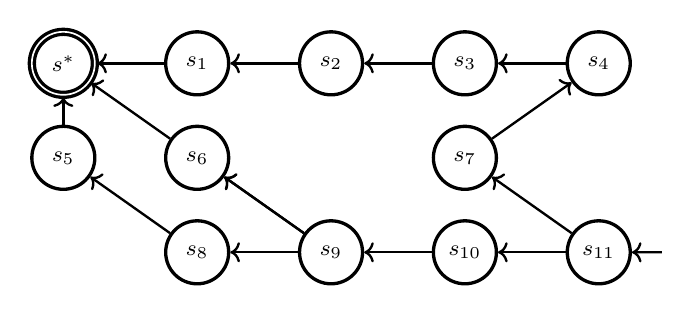
\begin{tikzpicture}
[
    node distance=12mm and 17mm, on grid, auto, label distance=-0.5mm,
    black_node/.style={circle, draw=black!100, fill=black!0, very thick, minimum height=8mm, minimum width=8mm},
]
    \node[black_node, accepting] (goal) {\footnotesize$s^*$} ;
    \node[black_node] (s1) [right = of goal] {\footnotesize$s_{1}$} ;
    \node[black_node] (s2) [right = of s1] {\footnotesize$s_{2}$} ;
    \node[black_node] (s3) [right = of s2] {\footnotesize$s_{3}$} ;
    \node[black_node] (s4) [right = of s3] {\footnotesize$s_{4}$} ;
    \node[black_node] (s5) [below = of goal] {\footnotesize$s_{5}$} ;
    \node[black_node] (s6) [below = of s1] {\footnotesize$s_{6}$} ;
    \node[black_node] (s7) [below = of s3] {\footnotesize$s_{7}$} ;
    \node[black_node] (s8) [below = of s6] {\footnotesize$s_{8}$} ;
    \node[black_node] (s9) [right = of s8] {\footnotesize$s_{9}$} ;
    \node[black_node] (s10) [right = of s9] {\footnotesize$s_{10}$} ;
    \node[black_node] (s11) [right = of s10] {\footnotesize$s_{11}$} ;
    \draw[->, line width=0.3mm, color=black] (s1) -- (goal) ;
    \draw[->, line width=0.3mm, color=black] (s2) -- (s1) ;
    \draw[->, line width=0.3mm, color=black] (s3) -- (s2) ;
    \draw[->, line width=0.3mm, color=black] (s4) -- (s3) ;
    \draw[->, line width=0.3mm, color=black] (s7) -- (s4) ;
    \draw[->, line width=0.3mm, color=black] (s11) -- (s7) ;
    \draw[->, line width=0.3mm, color=black] (s6) -- (goal) ;
    \draw[->, line width=0.3mm, color=black] (s9) -- (s6) ;
    \draw[->, line width=0.3mm, color=black] (s10) -- (s9) ;
    \draw[->, line width=0.3mm, color=black] (s11) -- (s10) ;
    \draw[->, line width=0.3mm, color=black] (s5) -- (goal) ;
    \draw[->, line width=0.3mm, color=black] (s8) -- (s5) ;
    \draw[->, line width=0.3mm, color=black] (s9) -- (s8) ;
    \draw[->, line width=0.3mm, color=black] (s9) -- (s6) ;
    \draw[->, line width=0.3mm, color=black] (7.6,-2.4) -- (s11) ;
\end{tikzpicture}
}
\only<2> {
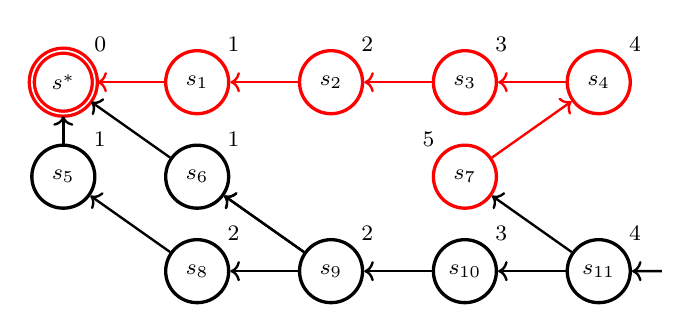
\begin{tikzpicture}
[
    node distance=12mm and 17mm, on grid, auto, label distance=-0.5mm,
    black_node/.style={circle, draw=black!100, fill=black!0, very thick, minimum height=8mm, minimum width=8mm},
    red_node/.style={circle, draw=red!100, fill=red!0, very thick, minimum height=8mm, minimum width=8mm},
]
    \node[red_node, accepting, label=above right:{\footnotesize$0$}] (goal) {\footnotesize$s^*$} ;
    \node[red_node, label=above right:{\footnotesize$1$}] (s1) [right = of goal] {\footnotesize$s_{1}$} ;
    \node[red_node, label=above right:{\footnotesize$2$}] (s2) [right = of s1] {\footnotesize$s_{2}$} ;
    \node[red_node, label=above right:{\footnotesize$3$}] (s3) [right = of s2] {\footnotesize$s_{3}$} ;
    \node[red_node, label=above right:{\footnotesize$4$}] (s4) [right = of s3] {\footnotesize$s_{4}$} ;
    \node[black_node, label=above right:{\footnotesize$1$}] (s5) [below = of goal] {\footnotesize$s_{5}$} ;
    \node[black_node, label=above right:{\footnotesize$1$}] (s6) [below = of s1] {\footnotesize$s_{6}$} ;
    \node[red_node, label=above left:{\footnotesize$5$}] (s7) [below = of s3] {\footnotesize$s_{7}$} ;
    \node[black_node, label=above right:{\footnotesize$2$}] (s8) [below = of s6] {\footnotesize$s_{8}$} ;
    \node[black_node, label=above right:{\footnotesize$2$}] (s9) [right = of s8] {\footnotesize$s_{9}$} ;
    \node[black_node, label=above right:{\footnotesize$3$}] (s10) [right = of s9] {\footnotesize$s_{10}$} ;
    \node[black_node, label=above right:{\footnotesize$4$}] (s11) [right = of s10] {\footnotesize$s_{11}$} ;
    \draw[->, line width=0.3mm, color=red] (s1) -- (goal) ;
    \draw[->, line width=0.3mm, color=red] (s2) -- (s1) ;
    \draw[->, line width=0.3mm, color=red] (s3) -- (s2) ;
    \draw[->, line width=0.3mm, color=red] (s4) -- (s3) ;
    \draw[->, line width=0.3mm, color=red] (s7) -- (s4) ;
    \draw[->, line width=0.3mm, color=black] (s11) -- (s7) ;
    \draw[->, line width=0.3mm, color=black] (s6) -- (goal) ;
    \draw[->, line width=0.3mm, color=black] (s9) -- (s6) ;
    \draw[->, line width=0.3mm, color=black] (s10) -- (s9) ;
    \draw[->, line width=0.3mm, color=black] (s11) -- (s10) ;
    \draw[->, line width=0.3mm, color=black] (s5) -- (goal) ;
    \draw[->, line width=0.3mm, color=black] (s8) -- (s5) ;
    \draw[->, line width=0.3mm, color=black] (s9) -- (s8) ;
    \draw[->, line width=0.3mm, color=black] (s9) -- (s6) ;
    \draw[->, line width=0.3mm, color=black] (7.6,-2.4) -- (s11) ;
\end{tikzpicture}
}
\end{center}
\pause
\begin{itemize}
    \item $\distfarthest=5$ from $s_7$.
    \begin{itemize}
        \item Regardless of the cost of operators!
    \end{itemize}
\end{itemize}
\end{frame}

\begin{frame}{Adaptative Regression Limit}
\begin{itemize}
    \item The ideal approach is a regression limit based on \distfarthest.
    \pause
    \begin{itemize}
        \item \distfarthest is unknown.
    \end{itemize}
    \pause
    \item Alternatively we can use task information.
    \bigskip \pause
    \item \textbf{Our proposals:} estimates the \distfarthest-value.
    \begin{itemize}
        \pause
        \item Number of facts: $\facts=|\mathcal{F}(s_0)|$
        \pause
        \item Number of facts per mean number of effects in the operators: $\meanfx=\ceil{L_F/\overline{\eff}}$ where $\overline{\eff}=\sum_{o\in \mathcal{O}} |\eff(o)|/|\mathcal{O}|$
    \end{itemize}
\end{itemize}
\end{frame}

\subsection{Randomly Generated Samples}

\begin{frame}{Randomly Generated Samples}
\begin{itemize}
    \item Regression may have difficulty reaching certain regions.
    \pause
    \item Randomly generated samples (\alert{random samples}) provide uniform coverage across the entire state space.
    \pause
    \item Adding random samples to the set of samples improves the performance of the learned heuristic \parencite{OToole/2022}.
    \begin{itemize}
        \item Generate a random state $s$ with cost-to-goal estimate $h(s) = max(H)+1$, where $H$ is the set of all cost-to-goal estimates in the original sample set.
    \end{itemize}
\end{itemize}
\end{frame}

\section{Cost-to-goal Estimates}

\begin{frame}{Cost-to-goal Estimates}
\begin{itemize}
    \item Based solely on the sampled rollout.

    \bigskip \pause
    
    \item How to improve?
    \begin{itemize}
        \item Use knowledge of all rollouts to update the sampled cost-to-goal estimate.
    \end{itemize}
\end{itemize}
\end{frame}


\subsection{Repeated Samples}

\begin{frame}{Sample Improvement}
\begin{itemize}
    \item A same state can be sampled by more than one rollout.
    \pause
    \item Repeated states can have different cost-to-goal estimates.
    \begin{itemize}
        \item Misinformation for NN learning.
    \end{itemize}
\end{itemize}
\bigskip \pause
\begin{itemize}
    \item \textbf{Our proposal:} for each sampled state $s$, update its cost-to-goal estimate to $h(s) = \min\{h_i \mid s=s_i, i\in[N]\}$.
    \begin{itemize}
        \item Never underestimate the perfect estimate $h^*$.
        \item This approach is called \alert{sample improvement} (SAI).
    \end{itemize}
\end{itemize}
\end{frame}

\begin{frame}{Sample Improvement}
\begin{columns}
\begin{column}{0.5\textwidth}
\centering
\only<1> {
    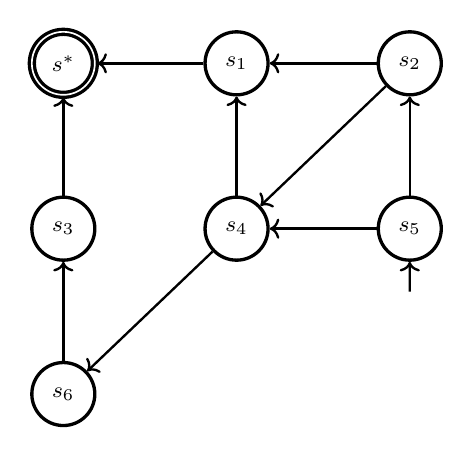
\begin{tikzpicture}
    [
        node distance=21mm and 22mm, on grid, auto, label distance=-0.5mm,
        black_node/.style={circle, draw=black!100, fill=black!0, very thick, minimum height=8mm, minimum width=8mm},
        red_node/.style={circle, draw=red!100, fill=red!0, very thick, minimum height=8mm, minimum width=8mm},
    ]
        \node[black_node, accepting] (goal) {\footnotesize$s^*$} ;
        \node[black_node] (s1) [right = of goal] {\footnotesize$s_{1}$} ;
        \node[black_node] (s2) [right = of s1] {\footnotesize$s_{2}$} ;
        \node[black_node] (s3) [below = of goal] {\footnotesize$s_{3}$} ;
        \node[black_node] (s4) [below = of s1] {\footnotesize$s_{4}$} ;
        \node[black_node] (s5) [below = of s2] {\footnotesize$s_{5}$} ;
        \node[black_node] (s6) [below = of s3] {\footnotesize$s_{6}$} ;
        \draw[->, line width=0.3mm, color=black] (s1) -- (goal) ;
        \draw[->, line width=0.3mm, color=black] (s2) -- (s1) ;
        \draw[->, line width=0.3mm, color=black] (s3) -- (goal) ;
        \draw[->, line width=0.3mm, color=black] (s6) -- (s3) ;
        \draw[->, line width=0.3mm, color=black] (s4) -- (s6) ;
        \draw[->, line width=0.3mm, color=black] (s4) -- (s1) ;
        \draw[->, line width=0.3mm, color=black] (s2) -- (s4) ;
        \draw[->, line width=0.3mm, color=black] (s5) -- (s2) ;
        \draw[->, line width=0.3mm, color=black] (s5) -- (s4) ;
        \draw[->, line width=0.3mm, color=black] (4.4,-2.9) -- (s5) ;
    \end{tikzpicture}
}
\only<2> {
    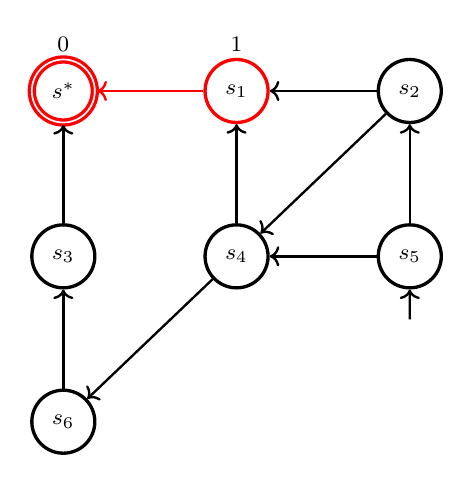
\begin{tikzpicture}
    [
        node distance=21mm and 22mm, on grid, auto, label distance=-0.5mm,
        black_node/.style={circle, draw=black!100, fill=black!0, very thick, minimum height=8mm, minimum width=8mm},
        red_node/.style={circle, draw=red!100, fill=red!0, very thick, minimum height=8mm, minimum width=8mm},
    ]
        \node[red_node, accepting, label=above:{\footnotesize$0$}] (goal) {\footnotesize$s^*$} ;
        \node[red_node, label=above:{\footnotesize$1$}] (s1) [right = of goal] {\footnotesize$s_{1}$} ;
        \node[black_node] (s2) [right = of s1] {\footnotesize$s_{2}$} ;
        \node[black_node] (s3) [below = of goal] {\footnotesize$s_{3}$} ;
        \node[black_node] (s4) [below = of s1] {\footnotesize$s_{4}$} ;
        \node[black_node] (s5) [below = of s2] {\footnotesize$s_{5}$} ;
        \node[black_node] (s6) [below = of s3] {\footnotesize$s_{6}$} ;
        \draw[->, line width=0.3mm, color=red] (s1) -- (goal) ;
        \draw[->, line width=0.3mm, color=black] (s2) -- (s1) ;
        \draw[->, line width=0.3mm, color=black] (s3) -- (goal) ;
        \draw[->, line width=0.3mm, color=black] (s6) -- (s3) ;
        \draw[->, line width=0.3mm, color=black] (s4) -- (s6) ;
        \draw[->, line width=0.3mm, color=black] (s4) -- (s1) ;
        \draw[->, line width=0.3mm, color=black] (s2) -- (s4) ;
        \draw[->, line width=0.3mm, color=black] (s5) -- (s2) ;
        \draw[->, line width=0.3mm, color=black] (s5) -- (s4) ;
        \draw[->, line width=0.3mm, color=black] (4.4,-2.9) -- (s5) ;
    \end{tikzpicture}
}
\only<3> {
    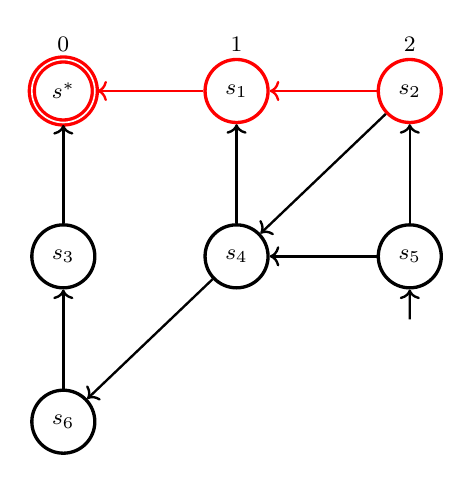
\begin{tikzpicture}
    [
        node distance=21mm and 22mm, on grid, auto, label distance=-0.5mm,
        black_node/.style={circle, draw=black!100, fill=black!0, very thick, minimum height=8mm, minimum width=8mm},
        red_node/.style={circle, draw=red!100, fill=red!0, very thick, minimum height=8mm, minimum width=8mm},
    ]
        \node[red_node, accepting, label=above:{\footnotesize$0$}] (goal) {\footnotesize$s^*$} ;
        \node[red_node, label=above:{\footnotesize$1$}] (s1) [right = of goal] {\footnotesize$s_{1}$} ;
        \node[red_node, label=above:{\footnotesize$2$}] (s2) [right = of s1] {\footnotesize$s_{2}$} ;
        \node[black_node] (s3) [below = of goal] {\footnotesize$s_{3}$} ;
        \node[black_node] (s4) [below = of s1] {\footnotesize$s_{4}$} ;
        \node[black_node] (s5) [below = of s2] {\footnotesize$s_{5}$} ;
        \node[black_node] (s6) [below = of s3] {\footnotesize$s_{6}$} ;
        \draw[->, line width=0.3mm, color=red] (s1) -- (goal) ;
        \draw[->, line width=0.3mm, color=red] (s2) -- (s1) ;
        \draw[->, line width=0.3mm, color=black] (s3) -- (goal) ;
        \draw[->, line width=0.3mm, color=black] (s6) -- (s3) ;
        \draw[->, line width=0.3mm, color=black] (s4) -- (s6) ;
        \draw[->, line width=0.3mm, color=black] (s4) -- (s1) ;
        \draw[->, line width=0.3mm, color=black] (s2) -- (s4) ;
        \draw[->, line width=0.3mm, color=black] (s5) -- (s2) ;
        \draw[->, line width=0.3mm, color=black] (s5) -- (s4) ;
        \draw[->, line width=0.3mm, color=black] (4.4,-2.9) -- (s5) ;
    \end{tikzpicture}
}
\only<4> {
    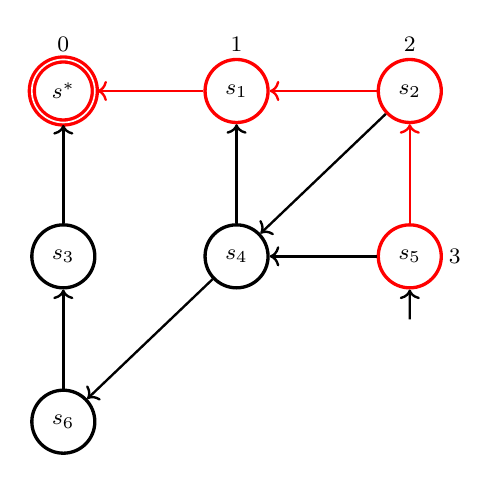
\begin{tikzpicture}
    [
        node distance=21mm and 22mm, on grid, auto, label distance=-0.5mm,
        black_node/.style={circle, draw=black!100, fill=black!0, very thick, minimum height=8mm, minimum width=8mm},
        red_node/.style={circle, draw=red!100, fill=red!0, very thick, minimum height=8mm, minimum width=8mm},
    ]
        \node[red_node, accepting, label=above:{\footnotesize$0$}] (goal) {\footnotesize$s^*$} ;
        \node[red_node, label=above:{\footnotesize$1$}] (s1) [right = of goal] {\footnotesize$s_{1}$} ;
        \node[red_node, label=above:{\footnotesize$2$}] (s2) [right = of s1] {\footnotesize$s_{2}$} ;
        \node[black_node] (s3) [below = of goal] {\footnotesize$s_{3}$} ;
        \node[black_node] (s4) [below = of s1] {\footnotesize$s_{4}$} ;
        \node[red_node, label=right:{\footnotesize$3$}] (s5) [below = of s2] {\footnotesize$s_{5}$} ;
        \node[black_node] (s6) [below = of s3] {\footnotesize$s_{6}$} ;
        \draw[->, line width=0.3mm, color=red] (s1) -- (goal) ;
        \draw[->, line width=0.3mm, color=red] (s2) -- (s1) ;
        \draw[->, line width=0.3mm, color=black] (s3) -- (goal) ;
        \draw[->, line width=0.3mm, color=black] (s6) -- (s3) ;
        \draw[->, line width=0.3mm, color=black] (s4) -- (s6) ;
        \draw[->, line width=0.3mm, color=black] (s4) -- (s1) ;
        \draw[->, line width=0.3mm, color=black] (s2) -- (s4) ;
        \draw[->, line width=0.3mm, color=red] (s5) -- (s2) ;
        \draw[->, line width=0.3mm, color=black] (s5) -- (s4) ;
        \draw[->, line width=0.3mm, color=black] (4.4,-2.9) -- (s5) ;
    \end{tikzpicture}
}
\only<5> {
    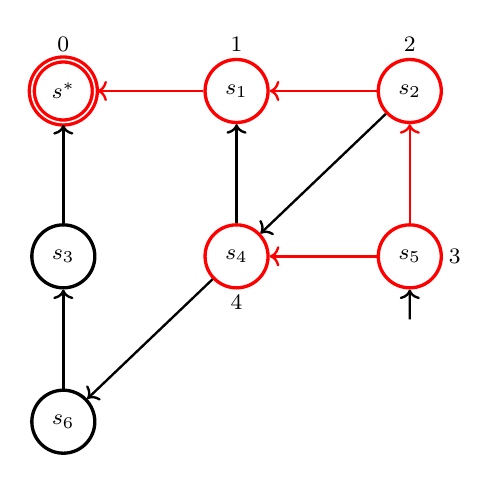
\begin{tikzpicture}
    [
        node distance=21mm and 22mm, on grid, auto, label distance=-0.5mm,
        black_node/.style={circle, draw=black!100, fill=black!0, very thick, minimum height=8mm, minimum width=8mm},
        red_node/.style={circle, draw=red!100, fill=red!0, very thick, minimum height=8mm, minimum width=8mm},
    ]
        \node[red_node, accepting, label=above:{\footnotesize$0$}] (goal) {\footnotesize$s^*$} ;
        \node[red_node, label=above:{\footnotesize$1$}] (s1) [right = of goal] {\footnotesize$s_{1}$} ;
        \node[red_node, label=above:{\footnotesize$2$}] (s2) [right = of s1] {\footnotesize$s_{2}$} ;
        \node[black_node] (s3) [below = of goal] {\footnotesize$s_{3}$} ;
        \node[red_node, label=below:{\footnotesize$4$}] (s4) [below = of s1] {\footnotesize$s_{4}$} ;
        \node[red_node, label=right:{\footnotesize$3$}] (s5) [below = of s2] {\footnotesize$s_{5}$} ;
        \node[black_node] (s6) [below = of s3] {\footnotesize$s_{6}$} ;
        \draw[->, line width=0.3mm, color=red] (s1) -- (goal) ;
        \draw[->, line width=0.3mm, color=red] (s2) -- (s1) ;
        \draw[->, line width=0.3mm, color=black] (s3) -- (goal) ;
        \draw[->, line width=0.3mm, color=black] (s6) -- (s3) ;
        \draw[->, line width=0.3mm, color=black] (s4) -- (s6) ;
        \draw[->, line width=0.3mm, color=black] (s4) -- (s1) ;
        \draw[->, line width=0.3mm, color=black] (s2) -- (s4) ;
        \draw[->, line width=0.3mm, color=red] (s5) -- (s2) ;
        \draw[->, line width=0.3mm, color=red] (s5) -- (s4) ;
        \draw[->, line width=0.3mm, color=black] (4.4,-2.9) -- (s5) ;
    \end{tikzpicture}
}
\only<6> {
    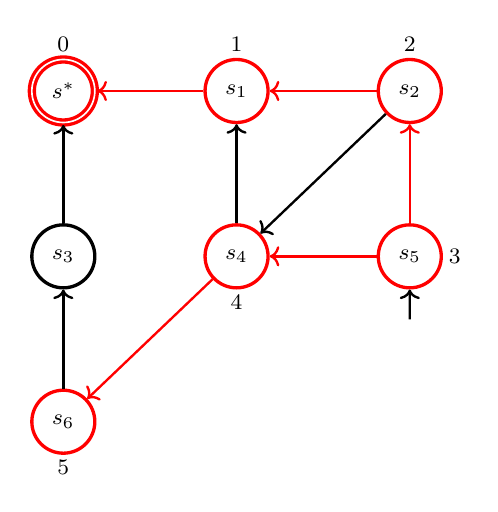
\begin{tikzpicture}
    [
        node distance=21mm and 22mm, on grid, auto, label distance=-0.5mm,
        black_node/.style={circle, draw=black!100, fill=black!0, very thick, minimum height=8mm, minimum width=8mm},
        red_node/.style={circle, draw=red!100, fill=red!0, very thick, minimum height=8mm, minimum width=8mm},
    ]
        \node[red_node, accepting, label=above:{\footnotesize$0$}] (goal) {\footnotesize$s^*$} ;
        \node[red_node, label=above:{\footnotesize$1$}] (s1) [right = of goal] {\footnotesize$s_{1}$} ;
        \node[red_node, label=above:{\footnotesize$2$}] (s2) [right = of s1] {\footnotesize$s_{2}$} ;
        \node[black_node] (s3) [below = of goal] {\footnotesize$s_{3}$} ;
        \node[red_node, label=below:{\footnotesize$4$}] (s4) [below = of s1] {\footnotesize$s_{4}$} ;
        \node[red_node, label=right:{\footnotesize$3$}] (s5) [below = of s2] {\footnotesize$s_{5}$} ;
        \node[red_node, label=below:{\footnotesize$5$}] (s6) [below = of s3] {\footnotesize$s_{6}$} ;
        \draw[->, line width=0.3mm, color=red] (s1) -- (goal) ;
        \draw[->, line width=0.3mm, color=red] (s2) -- (s1) ;
        \draw[->, line width=0.3mm, color=black] (s3) -- (goal) ;
        \draw[->, line width=0.3mm, color=black] (s6) -- (s3) ;
        \draw[->, line width=0.3mm, color=red] (s4) -- (s6) ;
        \draw[->, line width=0.3mm, color=black] (s4) -- (s1) ;
        \draw[->, line width=0.3mm, color=black] (s2) -- (s4) ;
        \draw[->, line width=0.3mm, color=red] (s5) -- (s2) ;
        \draw[->, line width=0.3mm, color=red] (s5) -- (s4) ;
        \draw[->, line width=0.3mm, color=black] (4.4,-2.9) -- (s5) ;
    \end{tikzpicture}
}
\only<7> {
    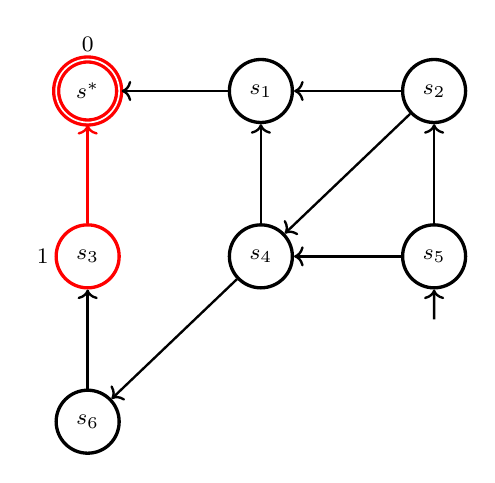
\begin{tikzpicture}
    [
        node distance=21mm and 22mm, on grid, auto, label distance=-0.5mm,
        black_node/.style={circle, draw=black!100, fill=black!0, very thick, minimum height=8mm, minimum width=8mm},
        red_node/.style={circle, draw=red!100, fill=red!0, very thick, minimum height=8mm, minimum width=8mm},
    ]
        \node[red_node, accepting, label=above:{\footnotesize$0$}] (goal) {\footnotesize$s^*$} ;
        \node[black_node] (s1) [right = of goal] {\footnotesize$s_{1}$} ;
        \node[black_node] (s2) [right = of s1] {\footnotesize$s_{2}$} ;
        \node[red_node, label=left:{\footnotesize$1$}] (s3) [below = of goal] {\footnotesize$s_{3}$} ;
        \node[black_node] (s4) [below = of s1] {\footnotesize$s_{4}$} ;
        \node[black_node] (s5) [below = of s2] {\footnotesize$s_{5}$} ;
        \node[black_node] (s6) [below = of s3] {\footnotesize$s_{6}$} ;
        \draw[->, line width=0.3mm, color=black] (s1) -- (goal) ;
        \draw[->, line width=0.3mm, color=black] (s2) -- (s1) ;
        \draw[->, line width=0.3mm, color=red] (s3) -- (goal) ;
        \draw[->, line width=0.3mm, color=black] (s6) -- (s3) ;
        \draw[->, line width=0.3mm, color=black] (s4) -- (s6) ;
        \draw[->, line width=0.3mm, color=black] (s4) -- (s1) ;
        \draw[->, line width=0.3mm, color=black] (s2) -- (s4) ;
        \draw[->, line width=0.3mm, color=black] (s5) -- (s2) ;
        \draw[->, line width=0.3mm, color=black] (s5) -- (s4) ;
        \draw[->, line width=0.3mm, color=black] (4.4,-2.9) -- (s5) ;
    \end{tikzpicture}
}
\only<8> {
    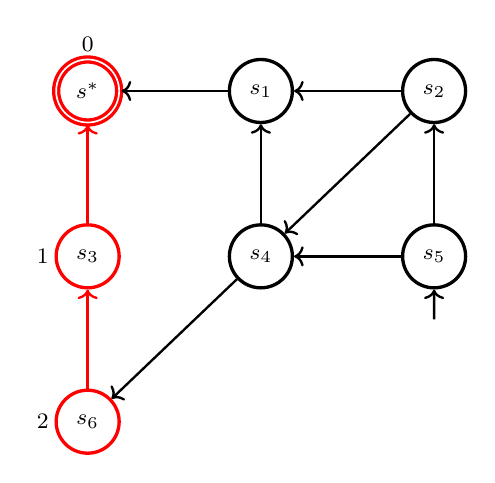
\begin{tikzpicture}
    [
        node distance=21mm and 22mm, on grid, auto, label distance=-0.5mm,
        black_node/.style={circle, draw=black!100, fill=black!0, very thick, minimum height=8mm, minimum width=8mm},
        red_node/.style={circle, draw=red!100, fill=red!0, very thick, minimum height=8mm, minimum width=8mm},
    ]
        \node[red_node, accepting, label=above:{\footnotesize$0$}] (goal) {\footnotesize$s^*$} ;
        \node[black_node] (s1) [right = of goal] {\footnotesize$s_{1}$} ;
        \node[black_node] (s2) [right = of s1] {\footnotesize$s_{2}$} ;
        \node[red_node, label=left:{\footnotesize$1$}] (s3) [below = of goal] {\footnotesize$s_{3}$} ;
        \node[black_node] (s4) [below = of s1] {\footnotesize$s_{4}$} ;
        \node[black_node] (s5) [below = of s2] {\footnotesize$s_{5}$} ;
        \node[red_node, label=left:{\footnotesize$2$}] (s6) [below = of s3] {\footnotesize$s_{6}$} ;
        \draw[->, line width=0.3mm, color=black] (s1) -- (goal) ;
        \draw[->, line width=0.3mm, color=black] (s2) -- (s1) ;
        \draw[->, line width=0.3mm, color=red] (s3) -- (goal) ;
        \draw[->, line width=0.3mm, color=red] (s6) -- (s3) ;
        \draw[->, line width=0.3mm, color=black] (s4) -- (s6) ;
        \draw[->, line width=0.3mm, color=black] (s4) -- (s1) ;
        \draw[->, line width=0.3mm, color=black] (s2) -- (s4) ;
        \draw[->, line width=0.3mm, color=black] (s5) -- (s2) ;
        \draw[->, line width=0.3mm, color=black] (s5) -- (s4) ;
        \draw[->, line width=0.3mm, color=black] (4.4,-2.9) -- (s5) ;
    \end{tikzpicture}
}
\only<9> {
    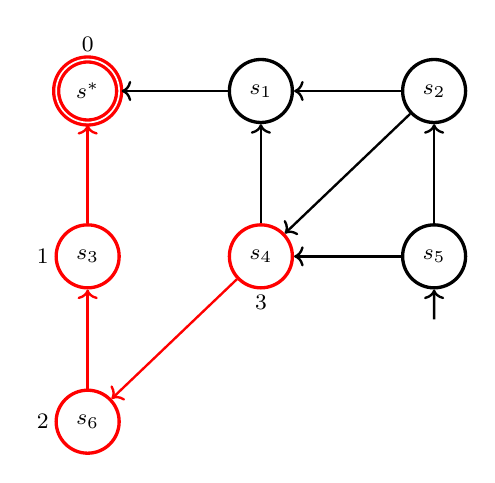
\begin{tikzpicture}
    [
        node distance=21mm and 22mm, on grid, auto, label distance=-0.5mm,
        black_node/.style={circle, draw=black!100, fill=black!0, very thick, minimum height=8mm, minimum width=8mm},
        red_node/.style={circle, draw=red!100, fill=red!0, very thick, minimum height=8mm, minimum width=8mm},
    ]
        \node[red_node, accepting, label=above:{\footnotesize$0$}] (goal) {\footnotesize$s^*$} ;
        \node[black_node] (s1) [right = of goal] {\footnotesize$s_{1}$} ;
        \node[black_node] (s2) [right = of s1] {\footnotesize$s_{2}$} ;
        \node[red_node, label=left:{\footnotesize$1$}] (s3) [below = of goal] {\footnotesize$s_{3}$} ;
        \node[red_node, label=below:{\footnotesize$3$}] (s4) [below = of s1] {\footnotesize$s_{4}$} ;
        \node[black_node] (s5) [below = of s2] {\footnotesize$s_{5}$} ;
        \node[red_node, label=left:{\footnotesize$2$}] (s6) [below = of s3] {\footnotesize$s_{6}$} ;
        \draw[->, line width=0.3mm, color=black] (s1) -- (goal) ;
        \draw[->, line width=0.3mm, color=black] (s2) -- (s1) ;
        \draw[->, line width=0.3mm, color=red] (s3) -- (goal) ;
        \draw[->, line width=0.3mm, color=red] (s6) -- (s3) ;
        \draw[->, line width=0.3mm, color=red] (s4) -- (s6) ;
        \draw[->, line width=0.3mm, color=black] (s4) -- (s1) ;
        \draw[->, line width=0.3mm, color=black] (s2) -- (s4) ;
        \draw[->, line width=0.3mm, color=black] (s5) -- (s2) ;
        \draw[->, line width=0.3mm, color=black] (s5) -- (s4) ;
        \draw[->, line width=0.3mm, color=black] (4.4,-2.9) -- (s5) ;
    \end{tikzpicture}
}
\only<10> {
    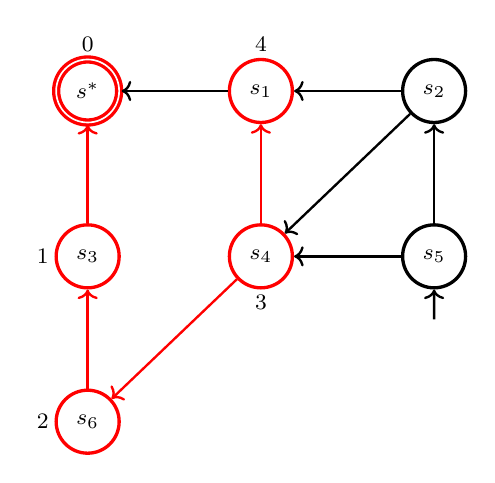
\begin{tikzpicture}
    [
        node distance=21mm and 22mm, on grid, auto, label distance=-0.5mm,
        black_node/.style={circle, draw=black!100, fill=black!0, very thick, minimum height=8mm, minimum width=8mm},
        red_node/.style={circle, draw=red!100, fill=red!0, very thick, minimum height=8mm, minimum width=8mm},
    ]
        \node[red_node, accepting, label=above:{\footnotesize$0$}] (goal) {\footnotesize$s^*$} ;
        \node[red_node, label=above:{\footnotesize$4$}] (s1) [right = of goal] {\footnotesize$s_{1}$} ;
        \node[black_node] (s2) [right = of s1] {\footnotesize$s_{2}$} ;
        \node[red_node, label=left:{\footnotesize$1$}] (s3) [below = of goal] {\footnotesize$s_{3}$} ;
        \node[red_node, label=below:{\footnotesize$3$}] (s4) [below = of s1] {\footnotesize$s_{4}$} ;
        \node[black_node] (s5) [below = of s2] {\footnotesize$s_{5}$} ;
        \node[red_node, label=left:{\footnotesize$2$}] (s6) [below = of s3] {\footnotesize$s_{6}$} ;
        \draw[->, line width=0.3mm, color=black] (s1) -- (goal) ;
        \draw[->, line width=0.3mm, color=black] (s2) -- (s1) ;
        \draw[->, line width=0.3mm, color=red] (s3) -- (goal) ;
        \draw[->, line width=0.3mm, color=red] (s6) -- (s3) ;
        \draw[->, line width=0.3mm, color=red] (s4) -- (s6) ;
        \draw[->, line width=0.3mm, color=red] (s4) -- (s1) ;
        \draw[->, line width=0.3mm, color=black] (s2) -- (s4) ;
        \draw[->, line width=0.3mm, color=black] (s5) -- (s2) ;
        \draw[->, line width=0.3mm, color=black] (s5) -- (s4) ;
        \draw[->, line width=0.3mm, color=black] (4.4,-2.9) -- (s5) ;
    \end{tikzpicture}
}
\only<11> {
    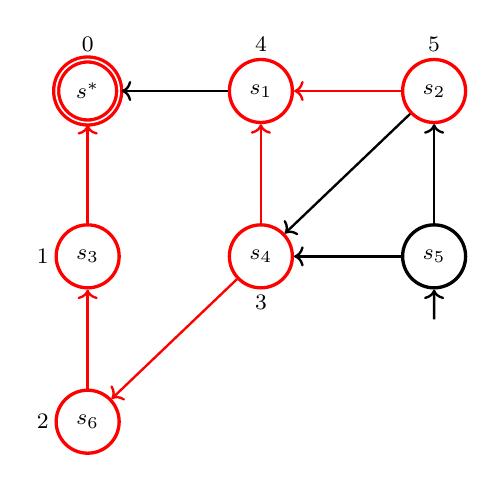
\begin{tikzpicture}
    [
        node distance=21mm and 22mm, on grid, auto, label distance=-0.5mm,
        black_node/.style={circle, draw=black!100, fill=black!0, very thick, minimum height=8mm, minimum width=8mm},
        red_node/.style={circle, draw=red!100, fill=red!0, very thick, minimum height=8mm, minimum width=8mm},
    ]
        \node[red_node, accepting, label=above:{\footnotesize$0$}] (goal) {\footnotesize$s^*$} ;
        \node[red_node, label=above:{\footnotesize$4$}] (s1) [right = of goal] {\footnotesize$s_{1}$} ;
        \node[red_node, label=above:{\footnotesize$5$}] (s2) [right = of s1] {\footnotesize$s_{2}$} ;
        \node[red_node, label=left:{\footnotesize$1$}] (s3) [below = of goal] {\footnotesize$s_{3}$} ;
        \node[red_node, label=below:{\footnotesize$3$}] (s4) [below = of s1] {\footnotesize$s_{4}$} ;
        \node[black_node] (s5) [below = of s2] {\footnotesize$s_{5}$} ;
        \node[red_node, label=left:{\footnotesize$2$}] (s6) [below = of s3] {\footnotesize$s_{6}$} ;
        \draw[->, line width=0.3mm, color=black] (s1) -- (goal) ;
        \draw[->, line width=0.3mm, color=red] (s2) -- (s1) ;
        \draw[->, line width=0.3mm, color=red] (s3) -- (goal) ;
        \draw[->, line width=0.3mm, color=red] (s6) -- (s3) ;
        \draw[->, line width=0.3mm, color=red] (s4) -- (s6) ;
        \draw[->, line width=0.3mm, color=red] (s4) -- (s1) ;
        \draw[->, line width=0.3mm, color=black] (s2) -- (s4) ;
        \draw[->, line width=0.3mm, color=black] (s5) -- (s2) ;
        \draw[->, line width=0.3mm, color=black] (s5) -- (s4) ;
        \draw[->, line width=0.3mm, color=black] (4.4,-2.9) -- (s5) ;
    \end{tikzpicture}
}
\only<12> {
\begin{itemize}
    \item $h(s^*)=min(0,0)=0$
    \item $h(s_1)=min(1,4)=1$
    \item $h(s_2)=min(2,5)=2$
    \item $h(s_3)=min(1)=1$
    \item $h(s_4)=min(4,3)=3$
    \item $h(s_5)=min(3)=3$
    \item $h(s_6)=min(5,2)=2$
\end{itemize}
}
\end{column}
\begin{column}{0.5\textwidth}
\only<1-11> {
    \begin{itemize}
        \pause
        \item Rollout \#1
        \begin{itemize}
            \item Sample \#1: $\langle s^*, 0 \rangle$
            \item Sample \#2: $\langle s_1, 1 \rangle$ \pause
            \item Sample \#3: $\langle s_2, 2 \rangle$ \pause
            \item Sample \#4: $\langle s_5, 3 \rangle$ \pause
            \item Sample \#5: $\langle s_4, 4 \rangle$ \pause
            \item Sample \#6: $\langle s_6, 5 \rangle$ \pause
        \end{itemize}
        \item Rollout \#2
        \begin{itemize}
            \item Sample \#7: $\langle s^*, 0 \rangle$
            \item Sample \#8: $\langle s_3, 1 \rangle$ \pause
            \item Sample \#9: $\langle s_6, 2 \rangle$ \pause
            \item Sample \#10: $\langle s_4, 3 \rangle$ \pause
            \item Sample \#11: $\langle s_1, 4 \rangle$ \pause
            \item Sample \#12: $\langle s_2, 5 \rangle$
        \end{itemize}
    \end{itemize}
}
\only<12> {
    \begin{itemize}
        \pause
        \item Rollout \#1
        \begin{itemize}
            \item Sample \#1: $\langle s^*, 0 \rangle$
            \item Sample \#2: $\langle s_1, 1 \rangle$
            \item Sample \#3: $\langle s_2, 2 \rangle$
            \item Sample \#4: $\langle s_5, 3 \rangle$
            \item Sample \#5: $\langle s_4, \text{\cancel{4}}\;\alert{3} \rangle$
            \item Sample \#6: $\langle s_6, \text{\cancel{5}}\;\alert{2} \rangle$
        \end{itemize}
        \item Rollout \#2
        \begin{itemize}
            \item Sample \#7: $\langle s^*, 0 \rangle$
            \item Sample \#8: $\langle s_3, 1 \rangle$
            \item Sample \#9: $\langle s_6, 2 \rangle$
            \item Sample \#10: $\langle s_4, 3 \rangle$
            \item Sample \#11: $\langle s_1, \text{\cancel{4}}\;\alert{1} \rangle$
            \item Sample \#12: $\langle s_2, \text{\cancel{5}}\;\alert{2} \rangle$
        \end{itemize}
    \end{itemize}
}
\end{column}
\end{columns}
\end{frame}

\subsection{Improvement over Successors}

\begin{frame}{Successors Improvement}
\begin{itemize}
    \item Multiple rollouts can generate neighboring (a distance operator) states in state space.

    \bigskip \pause
    
    \item \textbf{Our proposal:} Connect sampled states that are one operator away to create paths that generate knowledge to improve cost-to-goal estimates.
    \begin{itemize}
        \item This approach is called \alert{successors improvement} (SUI).
    \end{itemize}
\end{itemize}
\end{frame}

\begin{frame}{Successor Improvement}
\begin{columns}
\begin{column}{0.5\textwidth}
\only<1> {
    \begin{itemize}
        \item Rollout \#1
        \begin{itemize}
            \item Sample \#1: $\langle s^*, 0 \rangle$
            \item Sample \#2: $\langle s_3, 1 \rangle$
            \item Sample \#3: $\langle s_6, 2 \rangle$
            \item Sample \#4: $\langle s_4, 3 \rangle$
        \end{itemize}
    \end{itemize}
}
\only<2> {
    \begin{itemize}
        \item Rollout \#2
        \begin{itemize}
            \item Sample \#5: $\langle s^*, 0 \rangle$
            \item Sample \#6: $\langle s_1, 1 \rangle$
            \item Sample \#7: $\langle s_2, 2 \rangle$
            \item Sample \#8: $\langle s_4, 3 \rangle$
        \end{itemize}
    \end{itemize}
}
\only<3> {
    \begin{itemize}
        \item Rollout \#1
        \begin{itemize}
            \item Sample \#1: $\langle s^*, 0 \rangle$
            \item Sample \#2: $\langle s_3, 1 \rangle$
            \item Sample \#3: $\langle s_6, 2 \rangle$
            \item Sample \#4: $\langle s_4, 3 \rangle$
        \end{itemize}
        \item Rollout \#2
        \begin{itemize}
            \item Sample \#5: $\langle s^*, 0 \rangle$
            \item Sample \#6: $\langle s_1, 1 \rangle$
            \item Sample \#7: $\langle s_2, 2 \rangle$
            \item Sample \#8: $\langle s_4, 3 \rangle$
        \end{itemize}
    \end{itemize}
}
\only<4> {
    \begin{itemize}
        \item (1) Consider a directed graph $G=(V,A)$ over all sampled states, i.e.,~$V=\{s_i\mid i\in[N]\}$.
    \end{itemize}
}
\only<5> {
    \begin{itemize}
        \item (2) For every pair of states $s,t\in V$ such that for some operator $o\in\mathcal{O}$ applicable to $s$ we have $\text{succ}(s,o)\subseteq t$, we add an arc $(s,t)$ of length $\text{cost}(o)$ to $A$.
    \end{itemize}
}
\only<6> {
    \begin{itemize}
        \item (3) Propagates the cost-to-goal estimate of each state to its predecessors.
    \end{itemize}
}
\end{column}
\begin{column}{0.5\textwidth}
\only<1> {
    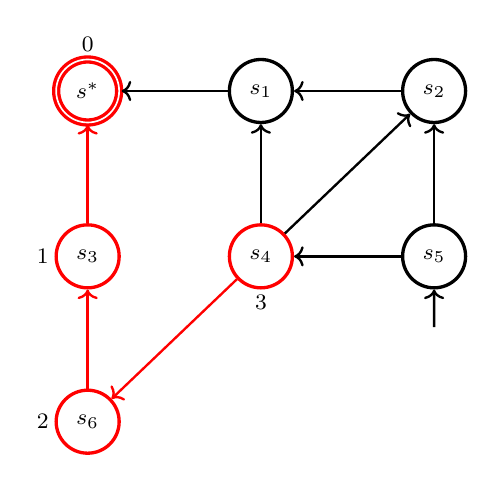
\begin{tikzpicture}
    [
        node distance=21mm and 22mm, on grid, auto, label distance=-0.5mm,
        black_node/.style={circle, draw=black!100, fill=black!0, very thick, minimum height=8mm, minimum width=8mm},
        red_node/.style={circle, draw=red!100, fill=red!0, very thick, minimum height=8mm, minimum width=8mm},
    ]
        \node[red_node, accepting, label=above:{\footnotesize$0$}] (goal) {\footnotesize$s^*$} ;
        \node[black_node] (s1) [right = of goal] {\footnotesize$s_{1}$} ;
        \node[black_node] (s2) [right = of s1] {\footnotesize$s_{2}$} ;
        \node[red_node, label=left:{\footnotesize$1$}] (s3) [below = of goal] {\footnotesize$s_{3}$} ;
        \node[red_node, label=below:{\footnotesize$3$}] (s4) [below = of s1] {\footnotesize$s_{4}$} ;
        \node[black_node] (s5) [below = of s2] {\footnotesize$s_{5}$} ;
        \node[red_node, label=left:{\footnotesize$2$}] (s6) [below = of s3] {\footnotesize$s_{6}$} ;
        \draw[->, line width=0.3mm, color=black] (s1) -- (goal) ;
        \draw[->, line width=0.3mm, color=black] (s2) -- (s1) ;
        \draw[->, line width=0.3mm, color=red] (s3) -- (goal) ;
        \draw[->, line width=0.3mm, color=red] (s6) -- (s3) ;
        \draw[->, line width=0.3mm, color=red] (s4) -- (s6) ;
        \draw[->, line width=0.3mm, color=black] (s4) -- (s1) ;
        \draw[->, line width=0.3mm, color=black] (s4) -- (s2) ;
        \draw[->, line width=0.3mm, color=black] (s5) -- (s2) ;
        \draw[->, line width=0.3mm, color=black] (s5) -- (s4) ;
        \draw[->, line width=0.3mm, color=black] (4.4,-3) -- (s5) ;
    \end{tikzpicture}
}
\only<2> {
    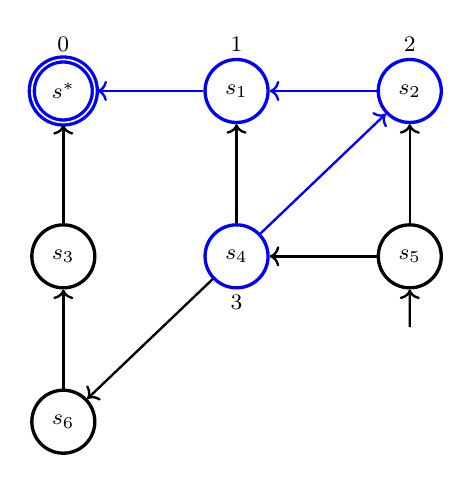
\begin{tikzpicture}
    [
        node distance=21mm and 22mm, on grid, auto, label distance=-0.5mm,
        black_node/.style={circle, draw=black!100, fill=black!0, very thick, minimum height=8mm, minimum width=8mm},
        blue_node/.style={circle, draw=blue!100, fill=blue!0, very thick, minimum height=8mm, minimum width=8mm},
    ]
        \node[blue_node, accepting, label=above:{\footnotesize$0$}] (goal) {\footnotesize$s^*$} ;
        \node[blue_node, label=above:{\footnotesize$1$}] (s1) [right = of goal] {\footnotesize$s_{1}$} ;
        \node[blue_node, label=above:{\footnotesize$2$}] (s2) [right = of s1] {\footnotesize$s_{2}$} ;
        \node[black_node] (s3) [below = of goal] {\footnotesize$s_{3}$} ;
        \node[blue_node, label=below:{\footnotesize$3$}] (s4) [below = of s1] {\footnotesize$s_{4}$} ;
        \node[black_node] (s5) [below = of s2] {\footnotesize$s_{5}$} ;
        \node[black_node] (s6) [below = of s3] {\footnotesize$s_{6}$} ;
        \draw[->, line width=0.3mm, color=blue] (s1) -- (goal) ;
        \draw[->, line width=0.3mm, color=blue] (s2) -- (s1) ;
        \draw[->, line width=0.3mm, color=black] (s3) -- (goal) ;
        \draw[->, line width=0.3mm, color=black] (s6) -- (s3) ;
        \draw[->, line width=0.3mm, color=black] (s4) -- (s6) ;
        \draw[->, line width=0.3mm, color=black] (s4) -- (s1) ;
        \draw[->, line width=0.3mm, color=blue] (s4) -- (s2) ;
        \draw[->, line width=0.3mm, color=black] (s5) -- (s2) ;
        \draw[->, line width=0.3mm, color=black] (s5) -- (s4) ;
        \draw[->, line width=0.3mm, color=black] (4.4,-3) -- (s5) ;
    \end{tikzpicture}
}
\only<3> {
    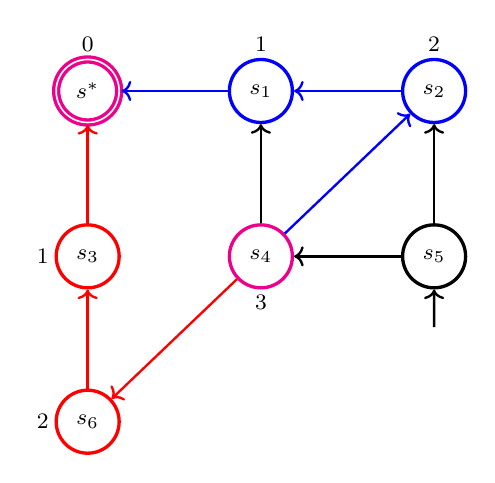
\begin{tikzpicture}
    [
        node distance=21mm and 22mm, on grid, auto, label distance=-0.5mm,
        black_node/.style={circle, draw=black!100, fill=black!0, very thick, minimum height=8mm, minimum width=8mm},
        red_node/.style={circle, draw=red!100, fill=red!0, very thick, minimum height=8mm, minimum width=8mm},
        blue_node/.style={circle, draw=blue!100, fill=blue!0, very thick, minimum height=8mm, minimum width=8mm},
        magenta_node/.style={circle, draw=magenta!100, fill=magenta!0, very thick, minimum height=8mm, minimum width=8mm},
    ]
        \node[magenta_node, accepting, label=above:{\footnotesize$0$}] (goal) {\footnotesize$s^*$} ;
        \node[blue_node, label=above:{\footnotesize$1$}] (s1) [right = of goal] {\footnotesize$s_{1}$} ;
        \node[blue_node, label=above:{\footnotesize$2$}] (s2) [right = of s1] {\footnotesize$s_{2}$} ;
        \node[red_node, label=left:{\footnotesize$1$}] (s3) [below = of goal] {\footnotesize$s_{3}$} ;
        \node[magenta_node, label=below:{\footnotesize$3$}] (s4) [below = of s1] {\footnotesize$s_{4}$} ;
        \node[black_node] (s5) [below = of s2] {\footnotesize$s_{5}$} ;
        \node[red_node, label=left:{\footnotesize$2$}] (s6) [below = of s3] {\footnotesize$s_{6}$} ;
        \draw[->, line width=0.3mm, color=blue] (s1) -- (goal) ;
        \draw[->, line width=0.3mm, color=blue] (s2) -- (s1) ;
        \draw[->, line width=0.3mm, color=red] (s3) -- (goal) ;
        \draw[->, line width=0.3mm, color=red] (s6) -- (s3) ;
        \draw[->, line width=0.3mm, color=red] (s4) -- (s6) ;
        \draw[->, line width=0.3mm, color=black] (s4) -- (s1) ;
        \draw[->, line width=0.3mm, color=blue] (s4) -- (s2) ;
        \draw[->, line width=0.3mm, color=black] (s5) -- (s2) ;
        \draw[->, line width=0.3mm, color=black] (s5) -- (s4) ;
        \draw[->, line width=0.3mm, color=black] (4.4,-3) -- (s5) ;
    \end{tikzpicture}
}
\only<4> {
    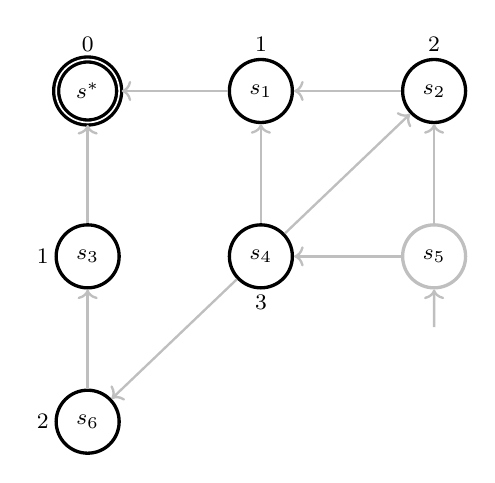
\begin{tikzpicture}
    [
        node distance=21mm and 22mm, on grid, auto, label distance=-0.5mm,
        black_node/.style={circle, draw=black!100, fill=black!0, very thick, minimum height=8mm, minimum width=8mm},
        grey_node/.style={circle, draw=lightgray, fill=black!0, very thick, minimum height=8mm, minimum width=8mm},
    ]
        \node[black_node, accepting, label=above:{\footnotesize$0$}] (goal) {\footnotesize$s^*$} ;
        \node[black_node, label=above:{\footnotesize$1$}] (s1) [right = of goal] {\footnotesize$s_{1}$} ;
        \node[black_node, label=above:{\footnotesize$2$}] (s2) [right = of s1] {\footnotesize$s_{2}$} ;
        \node[black_node, label=left:{\footnotesize$1$}] (s3) [below = of goal] {\footnotesize$s_{3}$} ;
        \node[black_node, label=below:{\footnotesize$3$}] (s4) [below = of s1] {\footnotesize$s_{4}$} ;
        \node[grey_node] (s5) [below = of s2] {\footnotesize$s_{5}$} ;
        \node[black_node, label=left:{\footnotesize$2$}] (s6) [below = of s3] {\footnotesize$s_{6}$} ;
        \draw[->, line width=0.3mm, color=lightgray] (s1) -- (goal) ;
        \draw[->, line width=0.3mm, color=lightgray] (s2) -- (s1) ;
        \draw[->, line width=0.3mm, color=lightgray] (s3) -- (goal) ;
        \draw[->, line width=0.3mm, color=lightgray] (s6) -- (s3) ;
        \draw[->, line width=0.3mm, color=lightgray] (s4) -- (s6) ;
        \draw[->, line width=0.3mm, color=lightgray] (s4) -- (s1) ;
        \draw[->, line width=0.3mm, color=lightgray] (s4) -- (s2) ;
        \draw[->, line width=0.3mm, color=lightgray] (s5) -- (s2) ;
        \draw[->, line width=0.3mm, color=lightgray] (s5) -- (s4) ;
        \draw[->, line width=0.3mm, color=lightgray] (4.4,-3) -- (s5) ;
    \end{tikzpicture}
}
\only<5> {
    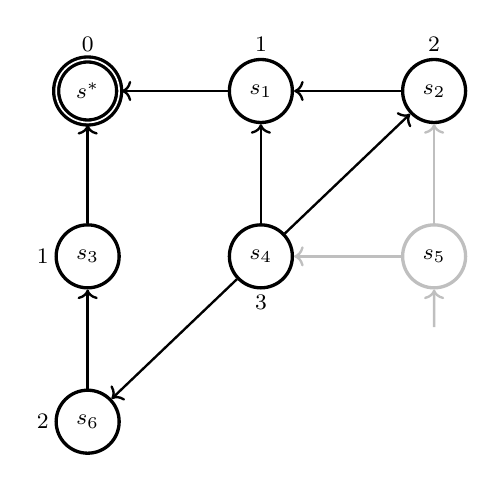
\begin{tikzpicture}
    [
        node distance=21mm and 22mm, on grid, auto, label distance=-0.5mm,
        black_node/.style={circle, draw=black!100, fill=black!0, very thick, minimum height=8mm, minimum width=8mm},
        grey_node/.style={circle, draw=lightgray, fill=black!0, very thick, minimum height=8mm, minimum width=8mm},
    ]
        \node[black_node, accepting, label=above:{\footnotesize$0$}] (goal) {\footnotesize$s^*$} ;
        \node[black_node, label=above:{\footnotesize$1$}] (s1) [right = of goal] {\footnotesize$s_{1}$} ;
        \node[black_node, label=above:{\footnotesize$2$}] (s2) [right = of s1] {\footnotesize$s_{2}$} ;
        \node[black_node, label=left:{\footnotesize$1$}] (s3) [below = of goal] {\footnotesize$s_{3}$} ;
        \node[black_node, label=below:{\footnotesize$3$}] (s4) [below = of s1] {\footnotesize$s_{4}$} ;
        \node[grey_node] (s5) [below = of s2] {\footnotesize$s_{5}$} ;
        \node[black_node, label=left:{\footnotesize$2$}] (s6) [below = of s3] {\footnotesize$s_{6}$} ;
        \draw[->, line width=0.3mm, color=black] (s1) -- (goal) ;
        \draw[->, line width=0.3mm, color=black] (s2) -- (s1) ;
        \draw[->, line width=0.3mm, color=black] (s3) -- (goal) ;
        \draw[->, line width=0.3mm, color=black] (s6) -- (s3) ;
        \draw[->, line width=0.3mm, color=black] (s4) -- (s6) ;
        \draw[->, line width=0.3mm, color=black] (s4) -- (s1) ;
        \draw[->, line width=0.3mm, color=black] (s4) -- (s2) ;
        \draw[->, line width=0.3mm, color=lightgray] (s5) -- (s2) ;
        \draw[->, line width=0.3mm, color=lightgray] (s5) -- (s4) ;
        \draw[->, line width=0.3mm, color=lightgray] (4.4,-3) -- (s5) ;
    \end{tikzpicture}
}
\only<6> {
    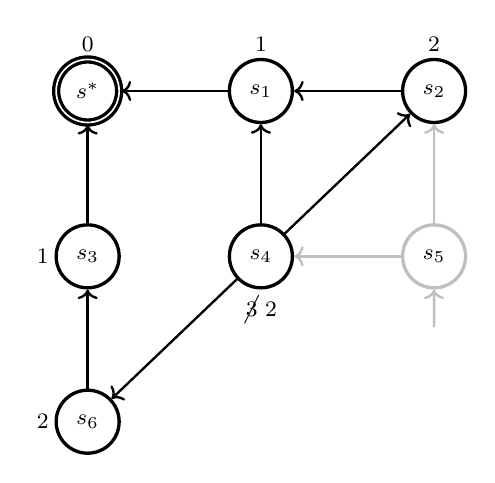
\begin{tikzpicture}
    [
        node distance=21mm and 22mm, on grid, auto, label distance=-0.5mm,
        black_node/.style={circle, draw=black!100, fill=black!0, very thick, minimum height=8mm, minimum width=8mm},
        grey_node/.style={circle, draw=lightgray, fill=black!0, very thick, minimum height=8mm, minimum width=8mm},
    ]
        \node[black_node, accepting, label=above:{\footnotesize$0$}] (goal) {\footnotesize$s^*$} ;
        \node[black_node, label=above:{\footnotesize$1$}] (s1) [right = of goal] {\footnotesize$s_{1}$} ;
        \node[black_node, label=above:{\footnotesize$2$}] (s2) [right = of s1] {\footnotesize$s_{2}$} ;
        \node[black_node, label=left:{\footnotesize$1$}] (s3) [below = of goal] {\footnotesize$s_{3}$} ;
        \node[black_node, label=below:{\footnotesize$\text{\cancel{3}}\;\alert{2}$}] (s4) [below = of s1] {\footnotesize$s_{4}$} ;
        \node[grey_node] (s5) [below = of s2] {\footnotesize$s_{5}$} ;
        \node[black_node, label=left:{\footnotesize$2$}] (s6) [below = of s3] {\footnotesize$s_{6}$} ;
        \draw[->, line width=0.3mm, color=black] (s1) -- (goal) ;
        \draw[->, line width=0.3mm, color=black] (s2) -- (s1) ;
        \draw[->, line width=0.3mm, color=black] (s3) -- (goal) ;
        \draw[->, line width=0.3mm, color=black] (s6) -- (s3) ;
        \draw[->, line width=0.3mm, color=black] (s4) -- (s6) ;
        \draw[->, line width=0.3mm, color=black] (s4) -- (s1) ;
        \draw[->, line width=0.3mm, color=black] (s4) -- (s2) ;
        \draw[->, line width=0.3mm, color=lightgray] (s5) -- (s2) ;
        \draw[->, line width=0.3mm, color=lightgray] (s5) -- (s4) ;
        \draw[->, line width=0.3mm, color=lightgray] (4.4,-3) -- (s5) ;
    \end{tikzpicture}
}
\end{column}
\end{columns}
\end{frame}


\section{Experiments}

\subsection{Settings}

\begin{frame}{Common Settings}
\begin{itemize}
    \item Same neural network architecture as \textcite{Ferber.etal/2022, OToole/2022}
    \begin{figure}
        \centering
        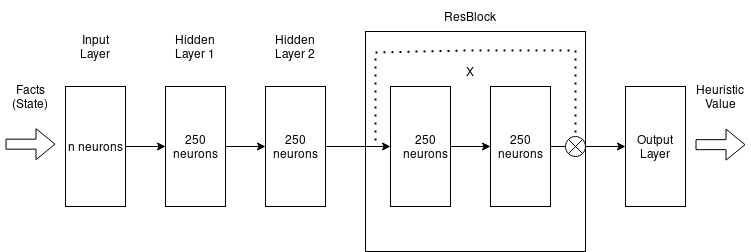
\includegraphics[width=9cm]{figures/resnet.png}
        \caption{Residual network.}
    \end{figure}
    \pause
    \item The experiments were divided into two parts: small state spaces and large state spaces.
    \pause
    \item Each task in the dataset has $50$ initial states.
    \pause
    \item Each experiment was run multiple times with different seeds.
\end{itemize}
\end{frame}

\begin{frame}{Baseline}
\begin{itemize}
    \item For comparative purposes, we experiment with a baseline configuration based on previous approaches from the literature.
    \pause
    \item The sampling method uses \alert{random walks} with a regression limit $L = 200$.
    \pause
    \item Improvement strategies SAI and SUI are turned off.
\end{itemize}
\end{frame}

\subsection{Small State Spaces}

\begin{frame}{Small State Spaces}
\begin{itemize}
    \item Tasks of the International Planning Competition (IPC) where the forward state space can be enumerated.
    \pause
    \begin{itemize}
        \item Allows the generation of all states in the state space and their perfect cost-to-goal estimates (\hstar).
        \pause
        \item Better control and understanding of the behavior of each technique.
    \end{itemize}
    \pause
    \item Number of samples $N$ equal to $1$\% of the total states of the forward state space.
    \pause
    \item All tasks are solved, so the number of expansions is used as the metric for the quality of the learned heuristic.
    \begin{itemize}
        \item \alert{Fewer expansions} means better heuristics!
    \end{itemize}
    \pause
    \item Domains and their state space sizes: Blocks (66K), Grid (452K), N-Puzzle (181K), Rovers (566K), Scanalyzer (46K), Transport (638K), and VisitAll (80K).
\end{itemize}
\end{frame}

\begin{frame}{Sampling Algorithm} % Table 3
\begin{table}[]
\begin{tabular}{l|rrrr}
    & \multicolumn{4}{c}{Expanded states} \\
    Sampling algorithm & BFS & DFS & RW & BFS+RW \\
    \hline
    Geo. mean & 446.72 & 326.66 & 79.78 & 73.12 \\
\end{tabular}
\end{table}
\begin{itemize}
    \pause
    \item BFS and DFS have extreme sample distributions. RW and our approach (BFS+RW) have a balanced sample distribution over the state space.
    \pause
    \item Blocks expands $5047$ states with BFS and Grid $4102$ with DFS, more than $25$ and $10$ times (resp.) than with the other techniques.
\end{itemize}
\end{frame}

\begin{frame}{Regression Limit} % Table 4
\begin{table}[]
\begin{tabular}{l|rrr}
    & \multicolumn{3}{c}{Expanded states} \\
    Regression Limit & \default & \facts & \meanfx \\
    \hline
    Geo. mean & 73.12 & 63.36 & 69.48 \\
\end{tabular}
\end{table}
\begin{itemize}
    \pause
    \item Our approaches outperform the baseline. \facts has the best performance, but...
    \pause
    \item \meanfx outperforms the other techniques in 4 of the 7 domains.
    \begin{itemize}
        \item Blocks expands $185$ states, more than twice as many as the other regression limits.
    \end{itemize}
\end{itemize}
\end{frame}

\begin{frame}{Random Samples} % Table 5
\begin{columns}
\begin{column}{0.5\textwidth}
    \begin{table}[]
    \begin{tabular}{l|rr}
        & \multicolumn{2}{c}{Expanded states} \\
        Domain & $0$\% & $20$\% \\
        \hline
        Blocks & 177.88 & \textbf{57.00} \\
        Grid & 124.89 & \textbf{66.52} \\
        N-Puzzle & 89.47 & \textbf{80.93} \\
        Rovers & 17.03 & \textbf{13.45} \\
        Scanalyzer & 55.29 & \textbf{28.34} \\
        Transport & \textbf{22.90} & 25.95 \\
        VisitAll & 30.90 & \textbf{21.78} \\
        \hline
        Geo. mean & 53.91 & 35.13 \\
    \end{tabular}
    \end{table}
\end{column}
\begin{column}{0.5\textwidth}
    \begin{itemize}
        \pause
        \item Improves performance up to $20$\% of random samples, then degrades.
        \pause
        \item Up to $50$\% of random samples the expanded states holds close ($35.13$~vs~$38.76$).
    \end{itemize}
\end{column}
\end{columns}
\end{frame}

\begin{frame}{Quality of Estimates (over the sample set)} % Table 7
\begin{columns}
\begin{column}{0.6\textwidth}  
    \begin{table}[]
    \begin{tabular}{l|rr}
        & \multicolumn{2}{c}{Mean difference \hstar-\hvalue} \\
        Domain & Baseline & Our approach \\
        \hline
        Blocks & 24.01 & 0.18 \\
        Grid & 13.60 & 0.61 \\
        N-Puzzle & 70.87 & 5.11 \\
        Rovers & 19.92 & 4.88 \\
        Scanalyzer & 81.35 & 1.89 \\
        Transport & 79.06 & 2.44 \\
        VisitAll & 15.80 & 2.15 \\
        \hline
        Geo. mean & 33.45 & 1.60 \\
    \end{tabular}
    \end{table}
\end{column}
\begin{column}{0.4\textwidth}
    \begin{itemize}
        \pause
        \item Our approach (BFS+RW, \meanfx, SAI and SUI) improves by $20$~times the approximation of the sample set estimates to \hstar.
        \pause
        \item Only \meanfx improves the mean difference to $5.56$. Only SAI and SUI improves to $10.95$.
    \end{itemize}
\end{column}
\end{columns}
\end{frame}

\begin{frame}{Quality of Estimates (over the forward state space)} % Table 8
\begin{columns}
\begin{column}{0.5\textwidth}
    \begin{table}[]
    \resizebox{\linewidth}{!}{
    \begin{tabular}{l|rr>{\onslide<2->}r<{\onslide}>{\onslide<3->}r<{\onslide}}
         & \multicolumn{4}{>{\onslide<1->}c<{\onslide}}{Mean difference \hstar-\hvalue} \\
        Domain & \hff & \hnnbase & \hnnbfsrwl{\meanfx} & \hnnrs \\
        \hline
        Blocks & 6.76 & 26.46 & 2.91 & 2.42 \\
        Grid & 3.72 & 26.85 & 2.73 & 9.78 \\
        N-Puzzle & 4.19 & 79.84 & 6.75 & 12.73 \\
        Rovers & 0.17 & 11.08 & 2.98 & 6.35 \\
        Scanalyzer & 2.78 & 106.37 & 2.99 & 9.01 \\
        Transport & 1.13 & 109.77 & 7.05 & 14.89 \\
        VisitAll & 1.31 & 21.55 & 2.21 & 4.74 \\
        \hline
        Geo. mean & 1.84 & 39.80 & 3.57 & 7.40 \\
    \end{tabular}}
    \end{table}
\end{column}
\begin{column}{0.5\textwidth}
    \begin{itemize}
        \item The mean difference \hstar-$h$ over the FS of baseline \hnnbase is more than $20$ times greater than \hff.
        \pause
        \item Our approach \hnnbfsrwl{\meanfx} improves considerably: close to \hff.
        \pause
        \item Adding random samples worsens the mean difference \hstar-$h$.
        \pause
        \begin{itemize}
            \item Improving the mean difference \hstar-$h$ doesn't necessarily reduce the expanded states...
        \end{itemize}
    \end{itemize}
\end{column}
\end{columns}
\end{frame}

\begin{frame}{Comparison of Heuristic Functions} % Table 9
\begin{table}[]
\begin{tabular}{l|r>{\onslide<2->}r<{\onslide}>{\onslide<3->}r<{\onslide}>{\onslide<4->}r<{\onslide}>{\onslide<5->}r<{\onslide}}
     & \multicolumn{5}{c}{Expanded states} \\
    Heuristic & \hstar & \hff & \hnnbase & \hnnbfsrwl{\meanfx} & \hnnrs \\
    \hline
    Geo. mean & 14.53 & 38.98 & 81.86 & 53.91 & 35.13 \\
\end{tabular}
\end{table}

\pause \pause \pause

\begin{itemize}
    \item Remains the relative order of quality of estimates over the FS.
    \pause
    \item But not. Random samples worsen the quality of estimates but reduce the expanded states.
    \pause
    \item Our approach with random samples (\hnnrs) outperforms \hff.
\end{itemize}
\end{frame}

\subsection{Large State Spaces}

\begin{frame}{Large State Spaces}
\begin{itemize}
    \item Validate our findings from experiments in small state spaces.
    \pause
    \item Fixed number of samples $N$ based on computational resources.
    \pause
    \item Coverage (percentage of solved tasks) is used as the metric for the quality of the learned heuristic.
    \begin{itemize}
        \item \alert{Greater coverage} means better heuristics!
    \end{itemize}
    \pause
    \item Dataset from \textcite{Ferber.etal/2022} moderate tasks.
    \begin{itemize}
        \item Domains and their number of tasks: Blocks (5), Depot\footnote[1]{Not in small state space experiments.} (6), Grid (2), N-Puzzle (8), Pipes-NT$^\text{\textbf{*}}$ (10), Rovers (8), Scanalyzer (6), Storage$^\text{\textbf{*}}$ (4), Transport (8), and VisitAll (6).
    \end{itemize}
\end{itemize}
\end{frame}

\begin{frame}{Comparison of Heuristic Functions (Coverage)} % Table 12
\begin{columns}
\begin{column}{0.5\textwidth}  
    \begin{table}[]
    \resizebox{\linewidth}{!}{
    \begin{tabular}{l|rrrr}
         & \multicolumn{4}{c}{Coverage (\%)} \\
        Domain & \hff & \hgc & \hnnbase & \hnnrs \\
        \hline
        Blocks & 100.00 & 100.00 & 100.00 & 100.00 \\
        Depot & 94.33 & 80.00 & 57.19 & 89.26 \\
        Grid & 94.00 & 51.00 & 38.11 & 60.33 \\
        N-Puzzle & 92.50 & 4.00 & 13.75 & 86.81 \\
        Pipes-NT & 63.40 & 89.40 & 13.51 & 79.84 \\
        Rovers & 85.50 & 66.00 & 13.53 & 15.39 \\
        Scanalyzer & 100.00 & 100.00 & 59.70 & 73.67 \\
        Storage & 33.00 & 13.50 & 1.94 & 27.67 \\
        Transport & 100.00 & 100.00 & 48.89 & 100.00 \\
        VisitAll & 92.00 & 100.00 & 74.19 & 98.85 \\
        \hline
        Mean & 85.47 & 70.39 & 42.08 & 73.18 \\
    \end{tabular}}
    \end{table}
\end{column}
\begin{column}{0.5\textwidth}
    \begin{itemize}
        \pause
        \item \hff dominates in most domains.
        \pause
        \item Our approach \hnnrs improves the baseline \hnnbase by about $31$\%, with competitive coverage in most domains.
        \pause
        \item Also, outperforms \hgc ($73.18$ vs $70.39$) with higher or equal coverage in $6$ out of $10$ domains.
    \end{itemize}
\end{column}
\end{columns}
\end{frame}

\begin{frame}{Comparison of Heuristic Functions (Expanded states)} % Table 12
\begin{columns}
\begin{column}{0.5\textwidth}  
    \begin{table}[]
    \resizebox{\linewidth}{!}{
    \begin{tabular}{l|rrrr}
         & \multicolumn{4}{c}{Expanded states} \\
        Domain & \hff & \hgc & \hnnbase & \hnnrs \\
        \hline
        Blocks & 36482 & 87026 & 5349 & 7335 \\
        Depot & 137053 & 874333 & 35972 & 29984 \\
        Grid & 45117 & 29990 & 15040 & 27009 \\
        N-Puzzle & - & - & - & - \\
        Pipes-NT & 83825 & 10416 & 304764 & 17389 \\
        Rovers & 38 & 466 & 596 & 30 \\
        Scanalyzer & 408 & 3914 & 27570 & 300 \\
        Storage & - & - & - & - \\
        Transport & 8342 & 253501 & 139311 & 12149 \\
        VisitAll & 248269 & 337 & 80155 & 5110 \\
        \hline
        Geo. mean & 12529 & 15706 & 25184 & 3937 \\
    \end{tabular}}
    \end{table}
\end{column}
\begin{column}{0.5\textwidth}
    \begin{itemize}
        \pause
        \item Our approach \hnnrs is the most informed on commonly solved tasks.
        \begin{itemize}
            \item Improves \hff by $3$ times.
        \end{itemize}
        \pause
        \item In all domains except Transport, our approach \hnnrs expands fewer states when compared to \hff.
        \pause
        \begin{itemize}
            \item Indicating that the lower coverage is an effect of the lower expansion speed of the NN-based heuristics.
        \end{itemize}
    \end{itemize}
\end{column}
\end{columns}
\end{frame}

\begin{frame}{Comparison to Other Methods} % Table 13
\begin{table}[]
\begin{tabular}{l|r}
    Technique & Avg. coverage \\
    \hline
    \hboot~\parencite{Ferber.etal/2022} & 45.40 \\
    \hnrsl~\parencite{OToole/2022} & 58.80 \\
    \hnnrs~(Our approach) & 72.82 \\
\end{tabular}
\end{table}
\bigskip
\begin{itemize}
    \pause
    \item All techniques use the same test dataset and NN architecture.
    \pause
    \item \hboot uses considerably more computational resources than the other techniques.
    \pause
    \item Our approach outperforms other techniques.
\end{itemize}
\end{frame}

\section{Conclusion}

\begin{frame}{Conclusion}
\begin{itemize}
    \pause
    \item For the samples obtained through regression, a distribution covering various portions of the state space without repeated samples close to the goal works best.
    \pause
    \item Both the sample size and reasonable cost-to-goal estimates contribute to search performance, with the latter being more important.
    \pause
    \item Fewer samples with more accurate $h$-values is better than having more samples with inaccurate $h$-values.
    \pause
    \item $h$-value improvement strategy SUI and adaptative rollout limit \meanfx have the most postiive impact on sampling quality.
    \pause
    \item Our approach outperforms \hgc but not \hff.
    \pause
    \begin{itemize}
        \item \hff has access to the entire model, whereas our approach only uses a minimal part of it.
    \end{itemize}
    \pause
    \item Approaches with few samples and computational resources can also be efficient.
\end{itemize}
\end{frame}

\printbibliography

\end{document}
